\def\fr{30}
\def\edg{边缘服务端}
\def\fr{10}
\def\acc{72.7\%}
\def\idenT{93毫秒}
\def\uiT{20秒}

\chapter{引言}\label{sec:introduction}

近年来,物联网(IoT)产业发展迅速。根据\cite{macgillivray2019worldwide},2025年将安装820亿台物联网设备。因此,人们有越来越多的机会与这些设备进行交互。物联网设备一般具有人可以操作的物理接口,例如按钮或开关。一种广泛接受的交互形式是使用应用程序通过另一个智能设备(如手机或笔记本电脑)来控制物联网设备\cite{homeass,xiaomi}。此外,通过语音命令进行交互也变得越来越流行\cite{li2019iot,porcheron2018voice}。与上述人机交互形式相比,增强现实(AR)技术能够直接在设备本体上显示出设备的信息和交互界面。因此,人们认为它有潜力打破物理空间和网络空间之间的界限。

在行业中,被最广泛接受的交互形式是使用一个手机应用程序(APP)来控制一组设备。这给用户带来了不便,用户必须自己链接物理和网络空间,也就是说,如果他们想要控制特定的设备,他们必须首先在应用程序的设备列表中找到相应的项目。

另一种新兴的交互式方法是语音交互。谷歌、亚马逊和苹果都设计并上市了他们的智能音箱,这些智能音箱可以通过WiFi等方式连接到家庭中所有可连接的设备。

语音交互在一定程度上减轻了用户的操作负担,因为他们只需说出自己的请求,而无需指明所要操作的设备。
然而,当交互目的变得复杂时,基于语音的交互同样会遇到物理与网络空间如何直观链接的问题。

Google Physical web\cite{jenson2014physical}为设备发现提供了一种更加自动化的方式,但它并没有解决设备的链接问题。

现有的一些工作试图通过类似AR的设计实现人机交互\cite{de2016snap,chen2018snaplink}。Snap-To-It\cite{de2016snap}允许用户通过拍摄设备照片并发送到服务器来选择设备。如果照片与某个设备匹配,服务器将返回该设备的控制界面并在手机上显示。SnapLink\cite{chen2018snaplink} 没有在识别设备时同时识别设备位置,但是也同样实现了对设备的控制。然而,他们只能在设备照片被拍摄后对该设备进行识别,这在速度上是不够的。\cite{liu2019edge} 研究了边缘辅助的实时移动增强现实技术,实现了高速移动中的增强现实技术。但是对于人机交互来说,\cite{liu2019edge} 缺乏识别设备的能力。\cite{ben2020edge,xu2020edge,liu2021edgesharing}提出的边缘辅助同步定位和地图构建(SLAM),实现了真正的实时SLAM。它们可以用于实现基于AR的人机交互,但还需要进一步的集成工作。

我们认为实现基于AR的人机交互有三个要求:1)视频帧中的设备应被准确识别和定位;2) 处理速度足够快,用户感觉不到延迟或掉帧;3) 交互以用户为导向,以提高体验质量。此外,我们注意到一个有趣的现象,即人们不仅希望与可连接的设备(即具有基本通信能力的设备)交互,而且希望与不可连接的对象进行交互。例如,用户希望保留培育植物的记录(例如浇水次数)。因此,我们希望将可连接/不可连接的对象都视为交互目标,将人与设备的交互进一步转化为人与对象的交互。

为了满足上述需求,我们提出了VSLink,它实现了快速的对象识别以及定制的交互这两项边缘服务。我们设计了一种两阶段目标识别方法,以保证识别的速度和准确性。两步目标识别方法利用视觉SLAM(Visual SLAM)和目标检测神经网络的互补特性,分别识别稳定/可移动的目标。Visual SLAM使用视觉特征点描述符来识别存储在地图中的稳定对象。在Visual SLAM过程之后,它生成一个检测的先验,表示存在对象的区域。通过稀疏卷积\cite{ren2018sbnet},神经网络的许多计算可以在这样的先验条件下被跳过,从而导致显著的推理加速。我们还为用户提供了一个平台,以实现面向用户的交互。使用该平台,用户可以自定义交互目标、功能和界面,而无需编码工作。


%A widely accepted interactive form in industries is to use a unified App to control a group of devices. This brings inconvenience that users have to link the physical and cyber space themselves, i.e., if they want to control a specific device, they have to find the corresponding item in the App's device list.
%Another rising interactive approach is through voice commands. Google, Amazon and Apple proposed their smart speakers which are linked to all connectable devices in a home. 
%To a certain extent, interaction through voice reduced the users' burden because 
%they can just tell their requests without naming a device.
%Nevertheless, voice based interaction will meet the link problem when the interactive purpose becomes complex.
%Google Physical web provides a more automatic way for device discovery, but it doesn't solve the link problem. 

学术界试图填补将物理和网络空间与先进技术联系起来的空白。
基于QR码的解决方案具有观察距离和角度的约束。
一些工作\cite{chen2018snaplink,de2016snap}要求用户拍摄目标设备的照片,然后分析照片以确定选择了哪个设备,这无法提供流畅的体验。一些工作\cite{alanwar2017selecon}需要在每个设备上部署传感节点,如UWB或RFID标签,这需要修改现有的物联网设备。
在这些工作中,\cite{chen2018snaplink}证明了将计算机视觉引入物理和网络空间目标之间的关联的有效性,但它们仍然存在局限性。
从系统灵活性的角度来看,它们缺乏用户定制交互体验的能力。
现有的实现大多需要开发人员设计交互API,这不够灵活。
在用户端,可以访问的设备、动作和数据都是固定的,不容易修改。
从用户体验的角度来看,快照活动限制了设备发现的速度,因为它要求用户按下快门并等待响应。想象一个用户来到一个新的地方,并寻找什么设备可以访问,这将需要大量的努力来保持周围的快照。
%Research fields have attempted to fill the gap of linking physical and cyber space with advanced technologies. 
%The QR code based solution has constraints of the looking distance and angle.
%Some~\cite{chen2018snaplink, de2016snap} request the user to take a photo of the target device and then analyzed the picture to identify which device is selected, which can't provide a fluent experience. Some~\cite{alanwar2017selecon} need to deploy sensing nodes such as UWB or RFID tags at each device, which requires modification of existing IoT devices. 


%Among these works, ~\cite{chen2018snaplink} proved the effectiveness of introducing computer vision for the association between targets in physical and cyber space, but they still have limitations. 
%From the system flexibility perspective, they lack the ability for the user to have customized interaction experience. 
%Existing implementations mostly require the developers to design the interaction API, which is not flexible enough. 
%In the user end, the device, action and data that can be accessed are settled and can't be easily modified.
%From the user experience perspective, snap activity limits the speed of device discovery since it asks the user to press the shutter and wait for a response. Imagining a user comes to a new place and looks for what devices can be accessed, it would take a lot of efforts to keep snapping around.
%
为了解决上述局限性,我们提出了VSLink,这是一种基于视觉SLAM的方法来连接物理和网络空间,它为用户提供了与环境对象的快速和普遍的交互。

在VSLink中,我们利用视觉SLAM来实时识别对象。这是因为SLAM将提供用户(即相机)的连续定位,这样我们就可以通过光线计算在智能手机屏幕上获得每个对象的坐标。

首先,我们为离线环境构建一个对象级映射。下次加载地图时,VSLink可以识别每个可见对象,并在屏幕上显示相应的API。

VSLink通过对象的位置和外观信息识别对象。这意味着,当物体移动时,我们能够使用视觉技术检测物体的出现/消失,并更新地图。为了加快识别物体出现/消失的过程,我们提出了一种结合视觉SLAM和物体检测神经网络的方法,该方法可以减少最先进模型(如YOLO和更快的RCNN)的计算量。VSLink还为用户提供与对象交互的通用模板。它非常灵活,易于修改,我们相信它会给用户带来更好的体验。
%To address the above limitations, we propose VSLink, which is a Visual SLAM based approach to link the physical and cyber space, and it provides the user a fast and pervasive interaction with environmental objects. 
%In VSLink, we take advantage of visual SLAM for identifying objects in a real time manner. This is because SLAM will offer a continuous localization of the user, i.e., the camera, such that we get each object's coordinate in the smartphone screen with light computation.
%At first, we build an object level map for the environment offline. Next time when the map is loaded, VSLink can identify every visible object and display the corresponding APIs on the screen. 
%VSLink recognizes an object via its location and appearance information. That means, when an object moves, we have the ability to detect the object's appearance/disappearance using vision techniques and update the map. To accelerate the process of identifying an object's appearance/disappearance, we propose a method that combines visual SLAM and object detection neural networks which could reduce the computation of state of the art models such as YOLO and Faster RCNN. VSLink also provides users common templates for interaction with objects. It's quite flexible and easy to modify, we believe it brings the user a better experience.

我们在包含20个对象的真实环境中评估了VSLink。结果表明,该系统支持30fps的视频输入,平均识别率为{\acc}。我们雇佣了10名志愿者通过VSLink实现他们的定制交互,结果表明,VSLink的使用、设计过程的平均时间成本在两分钟内。

本文的贡献总结如下:

1.我们提出了VSLink,这是一种基于AR的人机交互方法,融合了物理空间和网络空间。我们提出了一种两阶段目标识别方法来快速准确地识别目标。我们设计了一个平台来实现面向用户的交互定制。

2.我们实现了VSLink,并在包含多个对象的环境中对其进行了评估。结果表明,在支持30FPS视频输入的情况下,VSLink能实现实时运行。

本文的其余部分组织如下:第2节介绍了VSLink的框架。在第3节和第4节中,我们描述了两阶段目标识别方法和定制交互的设计。我们在第5节中介绍了VSLink的部署。在第6节中,我们介绍了相关的工作。我们在第8节中总结本文。

\begin{figure}[t]
	\centering
	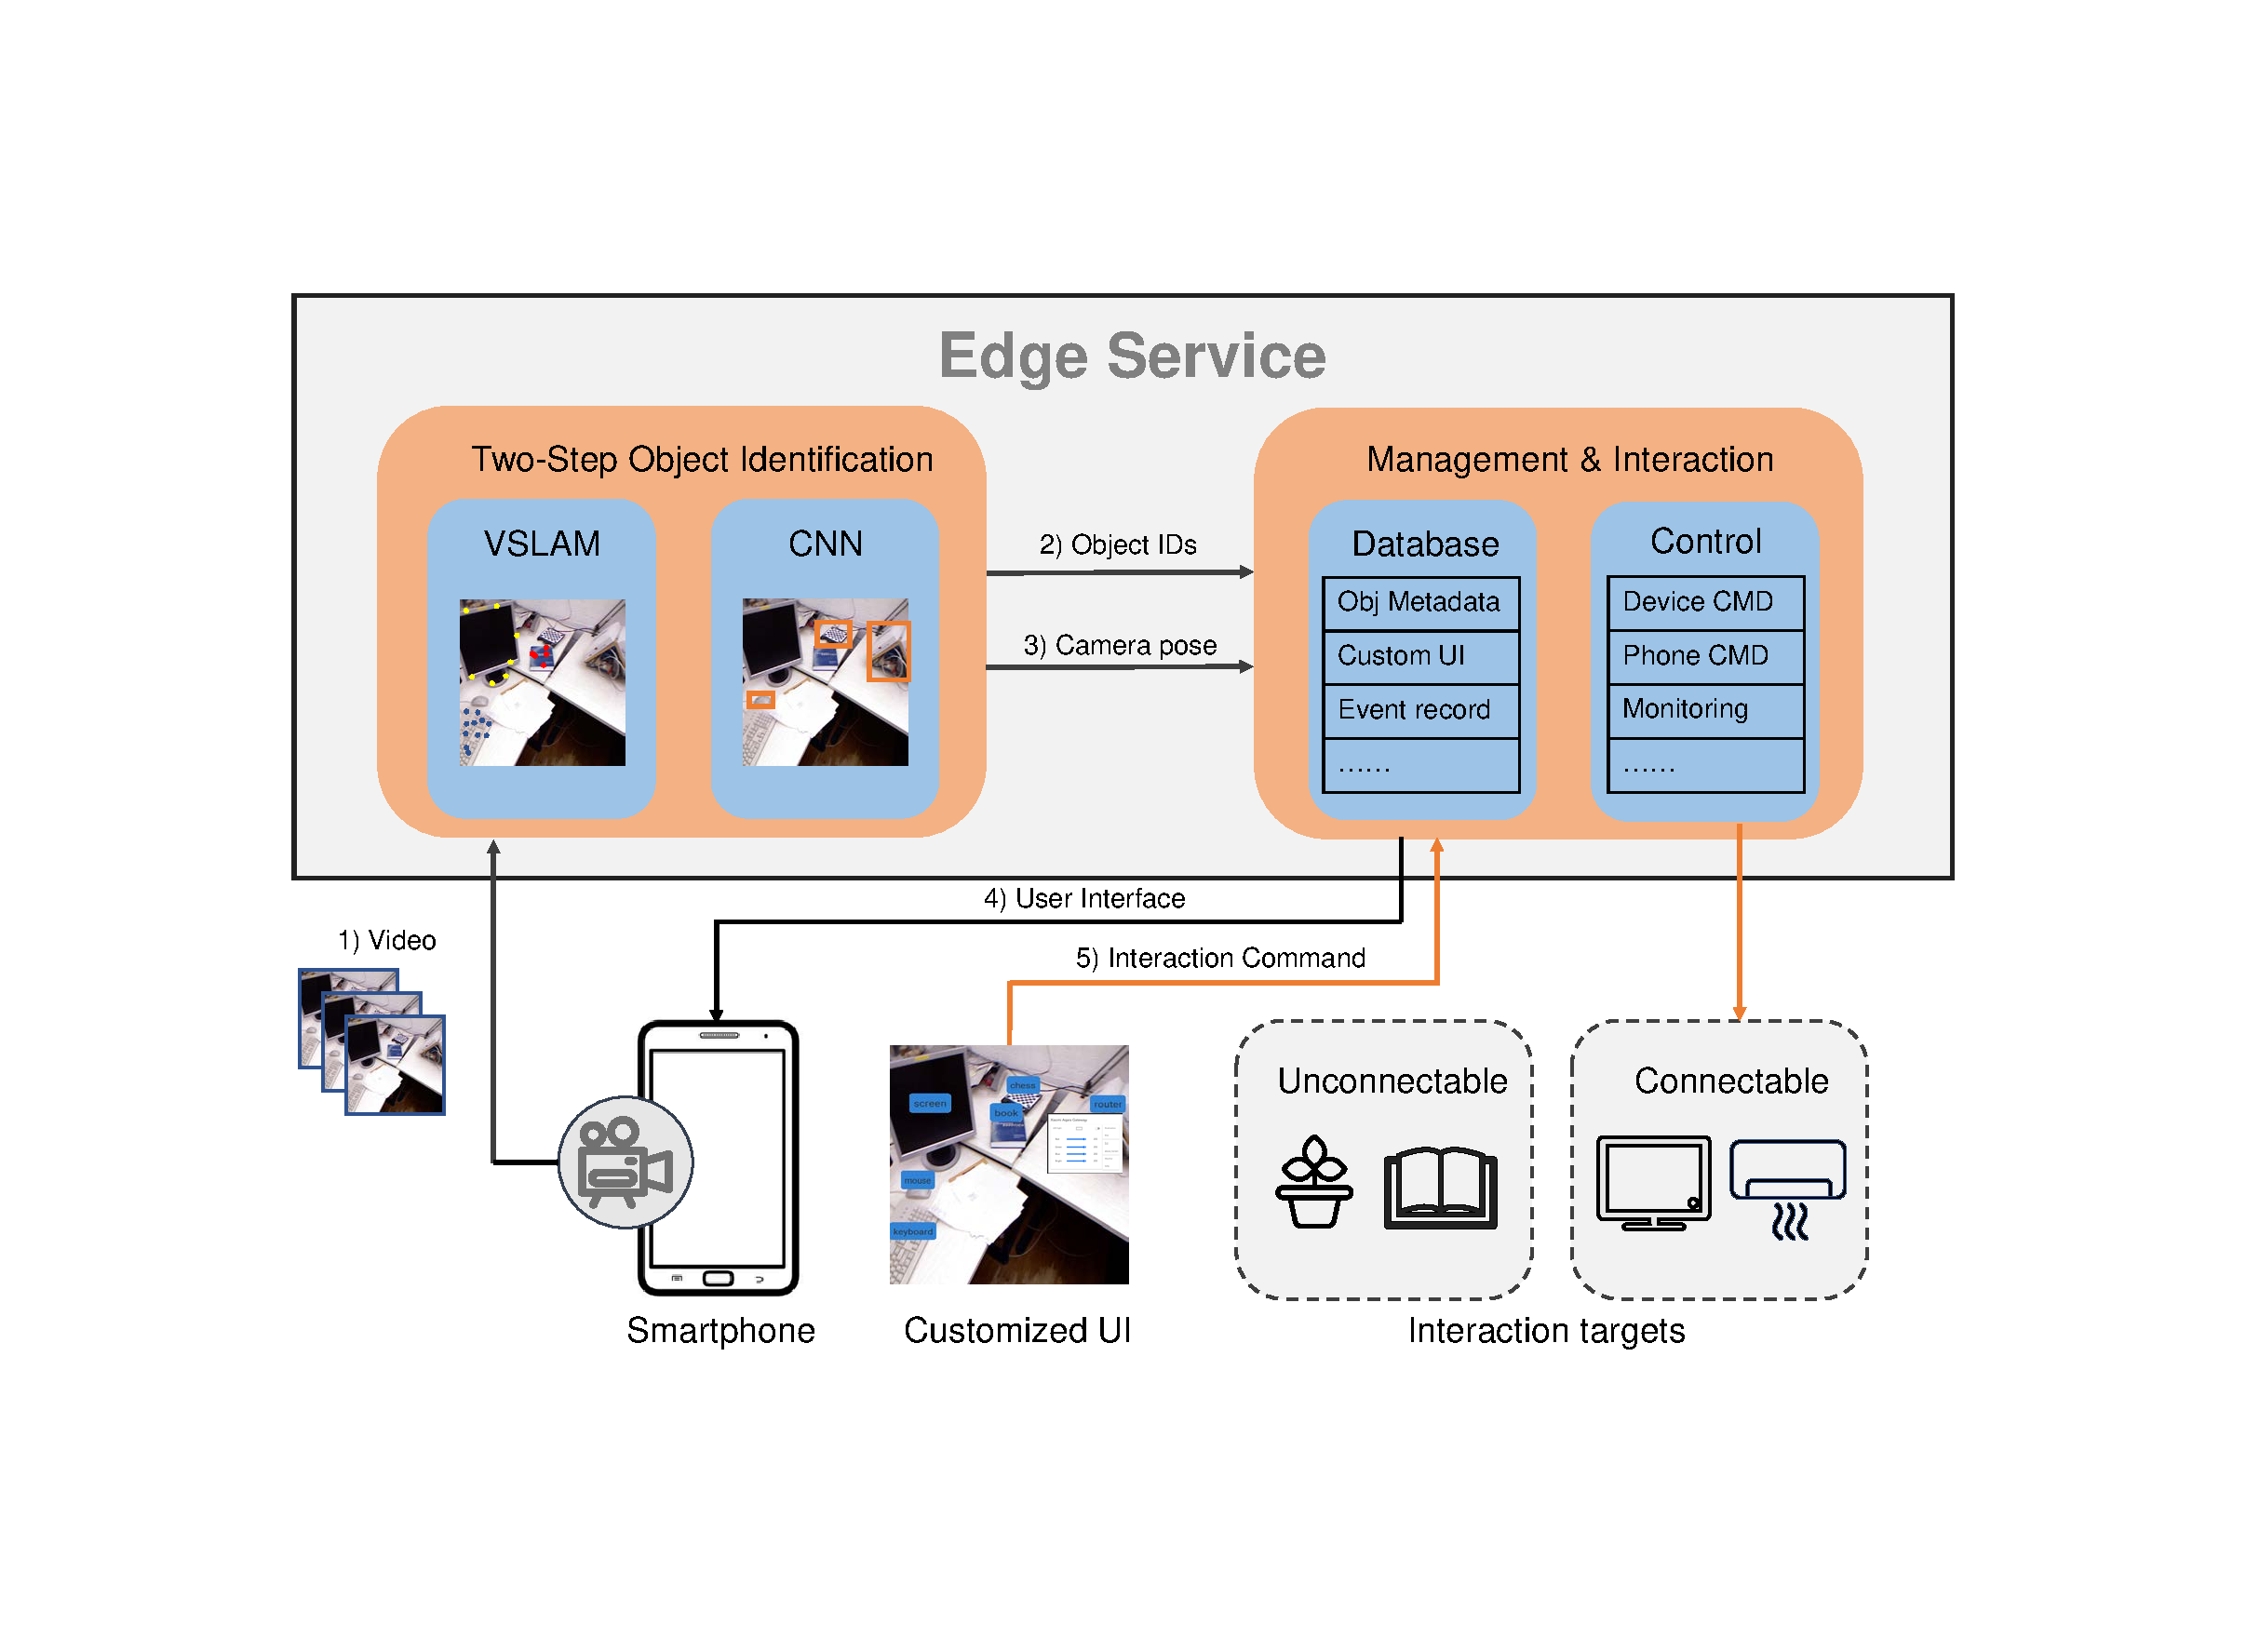
\includegraphics[width=0.99\linewidth]{overview}
	\caption{VSLink总体架构}
	\label{fig:overview}
\end{figure}

\chapter{系统架构}\label{sec:architec}


\autoref{fig:overview} 显示了我们提出的VSLink的体系结构:来自手机的视频帧被送往边缘服务,并将对应的UI送回手机端,用户可以使用UI进行交互。在高层次上,交互一共涉及到三端,即移动设备端、边缘服务端和对象端。我们可以将交互流程总结如下。首先,用户使用智能手机对周围环境进行视频监控,视频帧通过无线链路发送到边缘服务端。第二,边缘服务识别视频帧中的对象。相应的用户界面(UI)及其位置将发送到智能手机。第三,手机在对象的位置显示UI,用户通过操作UI输入交互命令。最后,该命令由对象/手机/边缘服务根据命令属性进行处理。

为了实现上述流程并实现用户体验的准确性、速度和质量的目标,在边缘服务端我们提出了两个模块,即两阶段目标识别和对象管理与交互。目标识别模块识别当前帧中的对象,并在较低延迟内返回其ID和位置。该模块借鉴Visual SLAM和目标检测神经网络的功能,实现快速准确的目标识别。具体来说,我们提前构建了环境的对象级SLAM映射。每次启动VSLink时,边缘服务端都会执行一个Visual SLAM线程。在通过构建的地图定位Visual SLAM的过程中,我们可以使用视觉特征点描述符匹配来识别位置稳定相对背景不动的对象。此外,为了处理移动目标,采用了目标检测神经网络。将Visual SLAM识别结果作为先验,提出了一种基于稀疏卷积的方法,避免了冗余计算。一旦一个物体被神经网络检测到,我们就使用图像检索方法来识别它的ID。

对象管理与交互模块实现了实际的人机交互。如果用户命令是由对象执行的,它会将用户命令发送给对象。例如,命令是打开某个设备。为了转发命令,边缘服务端与这些可连接对象建立连接,并集成它们的API。对于不可连接的对象,VSLink也提供了实现交互的功能,这主要依赖于智能手机的功能。

\chapter{两阶段目标识别}\label{sec:fast}
\section{动机}\label{subsec:motivation}
在计算机视觉领域,识别图像/视频中感兴趣的目标已经得到了很好的研究。例如,图像分类\cite{he2019bag}、目标检测\cite{zou2019object}、图像检索\cite{philbin2008lost,zheng2017sift}和图像定位\cite{sattler2011fast}可以实现不同程度的目标识别。在\autoref{table:methods}中,我们列出了这些方法的特点,但它们都不符合第\ref{sec:introduction}章中提到的要求。因此,我们将“目标检测+图像检索”方法与Visual SLAM相结合,以实现我们的目标识别。我们之所以选择这两种方法,是因为它们在许多方面表现出互补性。我们可以把环境中的物体大致分为两类,稳定的和可移动的。稳定物体往往位于固定位置,例如电视和空调。可移动的通常从一个地方移动到另一个地方。“对象检测+图像检索”方法(为了简化表示,我们在下面省略图像检索)能够识别所有对象,但由于需要经过神经网络运算,所以速度较慢,而Visual SLAM可以识别稳定对象且速度较快。

\autoref{fig:two-step-workflow}显示了所提出的两阶段目标识别方法的框架。这种设计接近于实际人脑的工作方式。例如,如果一个人进入卧室,她/他可以立即知道电视的位置,并对自己进行基本定位。然而,要识别手机,他需要集中注意力搜索。因此从直觉上来说,我们可以利用Visual SLAM的空间感知快速识别稳定的对象,然后让神经网络处理可能发生移动的对象。同时,神经网络不需要对整个图像进行分析,只需要对SLAM未识别的区域进行分析,可以大大减少时间开销。


\begin{table}[htbp]
    \centering
    \caption{\label{table:methods}现有目标识别解决方案的可行性}
    \begin{tabular}{|l|l|l|l|l|l|l|}\hline
    方法 &
      分类 &
      ID &
      多目标 &
      移动 &
      环境改变 &
      速度 \\
      \hline 图像分类\cite{he2019bag} &
      {\color[HTML]{355421} √} &
      {\color[HTML]{BF0000} ×} &
      {\color[HTML]{BF0000} ×} &
      {\color[HTML]{355421} √} &
      {\color[HTML]{355421} √} &
      {\color[HTML]{355421} 快} \\ \hline
    目标检测\cite{zou2019object} &
      {\color[HTML]{355421} √} &
      {\color[HTML]{BF0000} ×} &
      {\color[HTML]{355421} √} &
      {\color[HTML]{355421} √} &
      {\color[HTML]{355421} √} &
      {\color[HTML]{BF0000} 慢} \\ \hline
    图像检索\cite{philbin2008lost,zheng2017sift} &
      {\color[HTML]{BF0000} ×} &
      {\color[HTML]{355421} √} &
      {\color[HTML]{BF0000} ×} &
      {\color[HTML]{355421} √} &
      {\color[HTML]{355421} √} &
      {\color[HTML]{355421} 快} \\ \hline
    检测+检索 &
      {\color[HTML]{355421} √} &
      {\color[HTML]{355421} √} &
      {\color[HTML]{355421} √} &
      {\color[HTML]{355421} √} &
      {\color[HTML]{355421} √} &
      {\color[HTML]{BF0000} 慢} \\ \hline
    图像定位\cite{sattler2011fast} &
      {\color[HTML]{BF0000} ×} &
      {\color[HTML]{355421} √} &
      {\color[HTML]{355421} √} &
      {\color[HTML]{BF0000} ×} &
      {\color[HTML]{BF0000} ×} &
      {\color[HTML]{BF0000} 慢} \\ \hline
    Visual SLAM\cite{liu2021edgesharing} &
      {\color[HTML]{BF0000} ×} &
      {\color[HTML]{355421} √} &
      {\color[HTML]{355421} √} &
      {\color[HTML]{BF0000} ×} &
      {\color[HTML]{BF0000} ×} &
      {\color[HTML]{355421} 快} \\ \hline
    \end{tabular}
    \end{table}

    \begin{figure}[t]
        \centering
        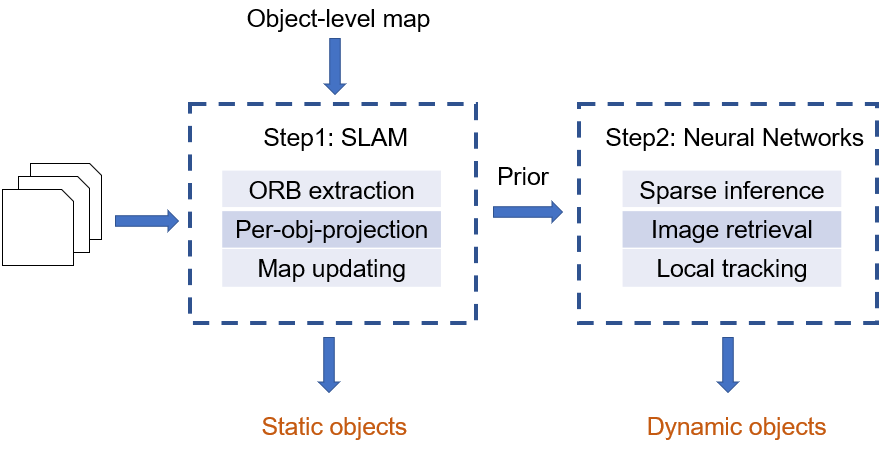
\includegraphics[width=0.75\linewidth]{twostep}
        \caption{两阶段目标识别方法框架}
        \label{fig:two-step-workflow}
    \end{figure}

    \begin{figure}[t]
        \centering
        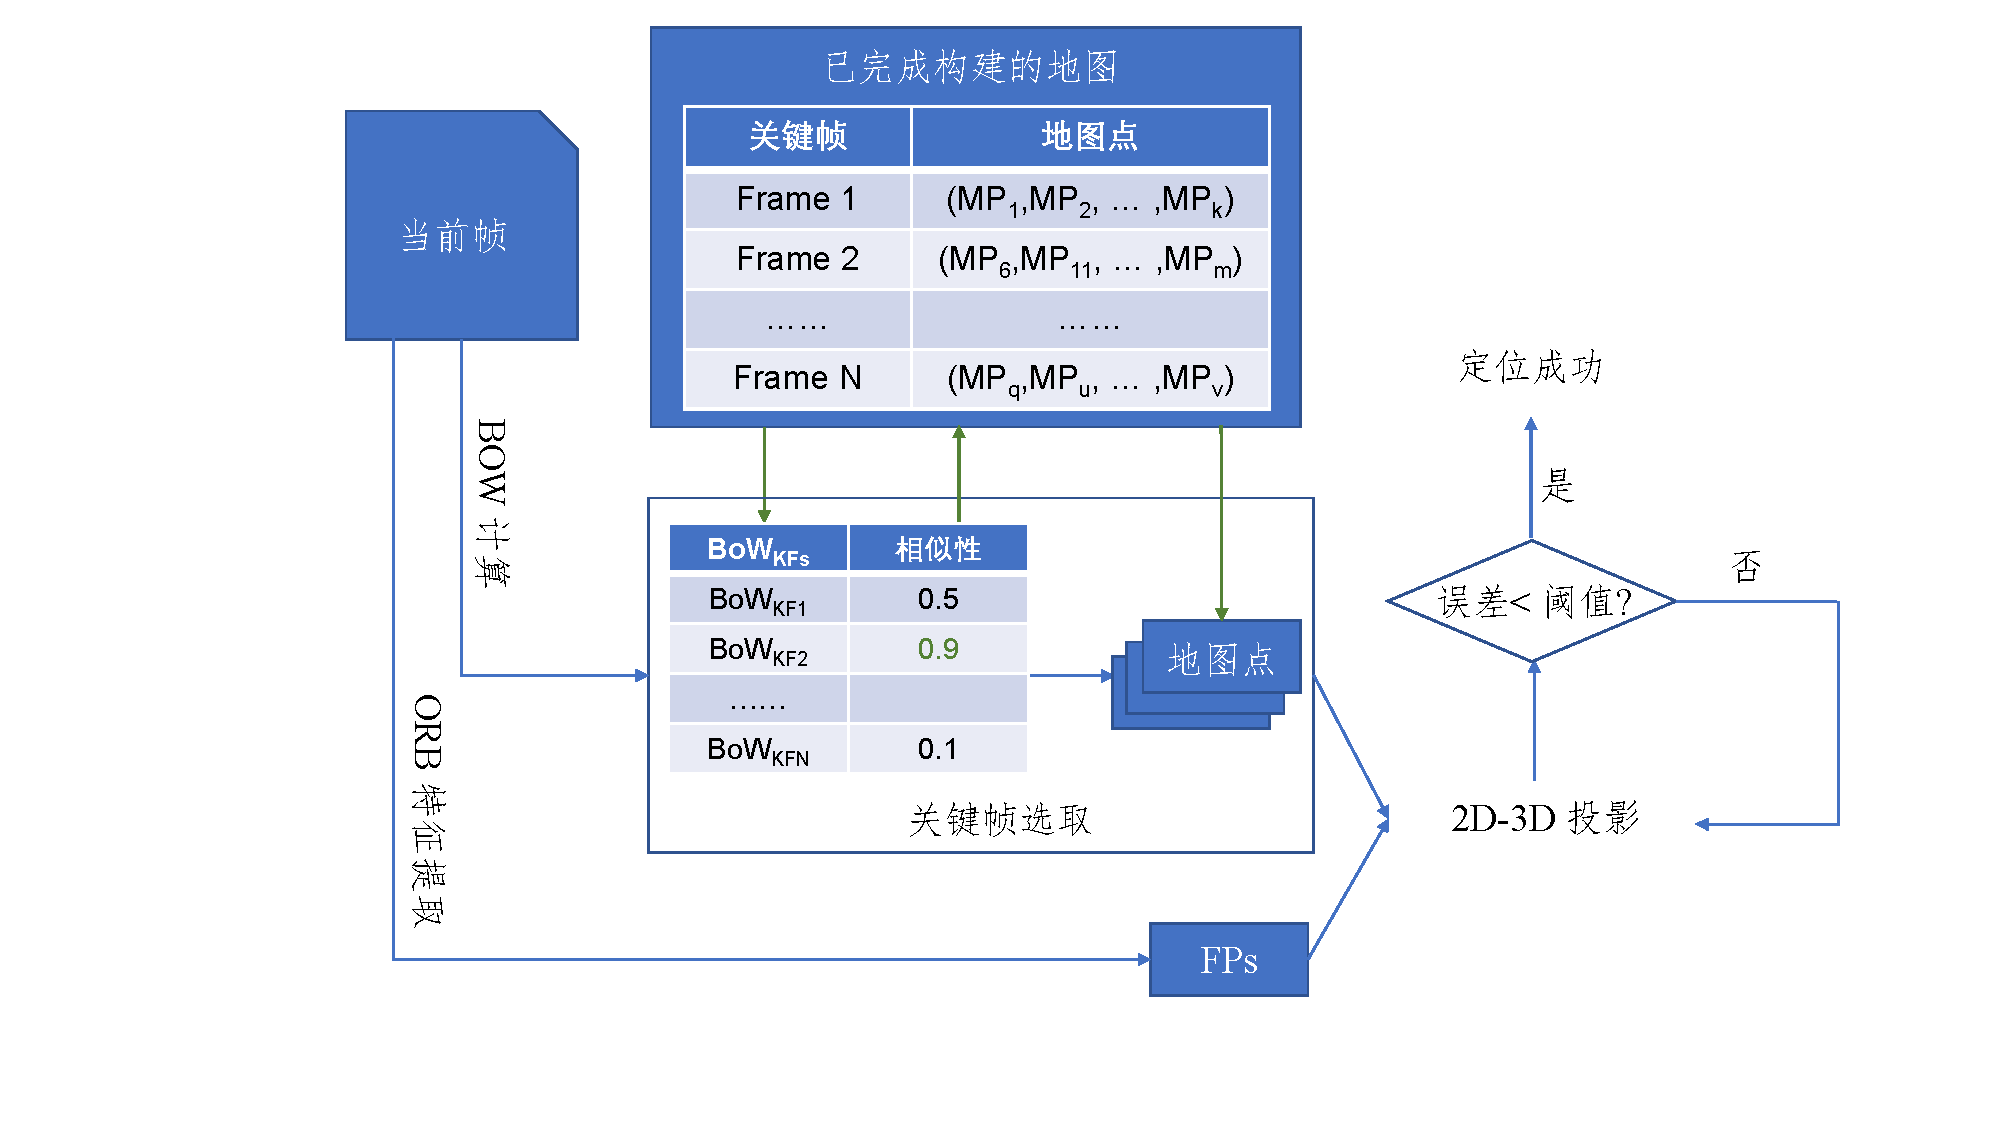
\includegraphics[width=0.8\linewidth]{workflow}
        \caption{ORB-SLAM\cite{mur2017orb}在地图重用时的定位过程}
        \label{fig:localization}
    \end{figure}
\section{基于Visual SLAM的目标识别}\label{subsec:vslam}
SLAM被认为是实现更真实AR体验的关键技术之一,因为它提供了对环境的理解和跟踪。在VSLink中,我们建立了一个终身对象级SLAM映射,这有利于SLAM跟踪和对象识别。

\subsection{工作流程}
在这里,我们解释了所提出的基于Visual SLAM的对象识别解决方案的理论。由于经典的Visual SLAM\cite{mur2017orb,engel2014lsd}技术试图在机器人第一次进入环境时实现精确的映射和定位,我们想知道机器人第二次进入环境时是否能够识别它所看到的物体。

构建的SLAM地图\cite{mur2017orb}仅包括某些地图点和关键帧,地图重用过程如图3所示。定位过程首先使用单词包(BoW)\cite{galvez2012bags}计算当前帧的表示,然后计算当前帧和关键帧之间的BoW相似性。然后,它选择具有高弓相似性的关键帧作为候选帧。最后,对于每个选定的关键帧,它使用RANSAC\cite{derpanis2010overview}算法计算当前帧中的特征点与该关键帧的贴图点之间的2D-3D投影。如果投影误差小于阈值,则定位完成。

我们注意到,上述过程的实质是在地图点$mp = [x_m,y_m,z_m,\vec{orb}]$(在重用的地图中)和特征点$fp = [x_f,y_f,\vec{orb}]$(在当前框架中)之间建立投影,其中下标$m$和$f$表示地图坐标系和框架坐标系。
因此,如果我们给$mp$一个表示对象ID的标签,并且在本地化期间将该$mp$投影到某个$fp$,则相应的对象将在当前帧中本地化。
与原始VSLAM相比,在标记贴图点后,我们能够在不引入额外计算的情况下识别环境中的对象。
请注意,此方法不只是记住对象的位置,当对象相对于其在地图上的位置移动时,可能会导致误报检测。
ORB特征用于建立2D-3D投影,这意味着SLAM在环境中定位自身后,当某些特征点可见时,它会识别到对象。
虽然不常见,但是我们也考虑了稳定物体移动的情况,我们使用了逐对象投影算法来检测这种运动并更新地图。


\begin{figure}[t]
	\centering
	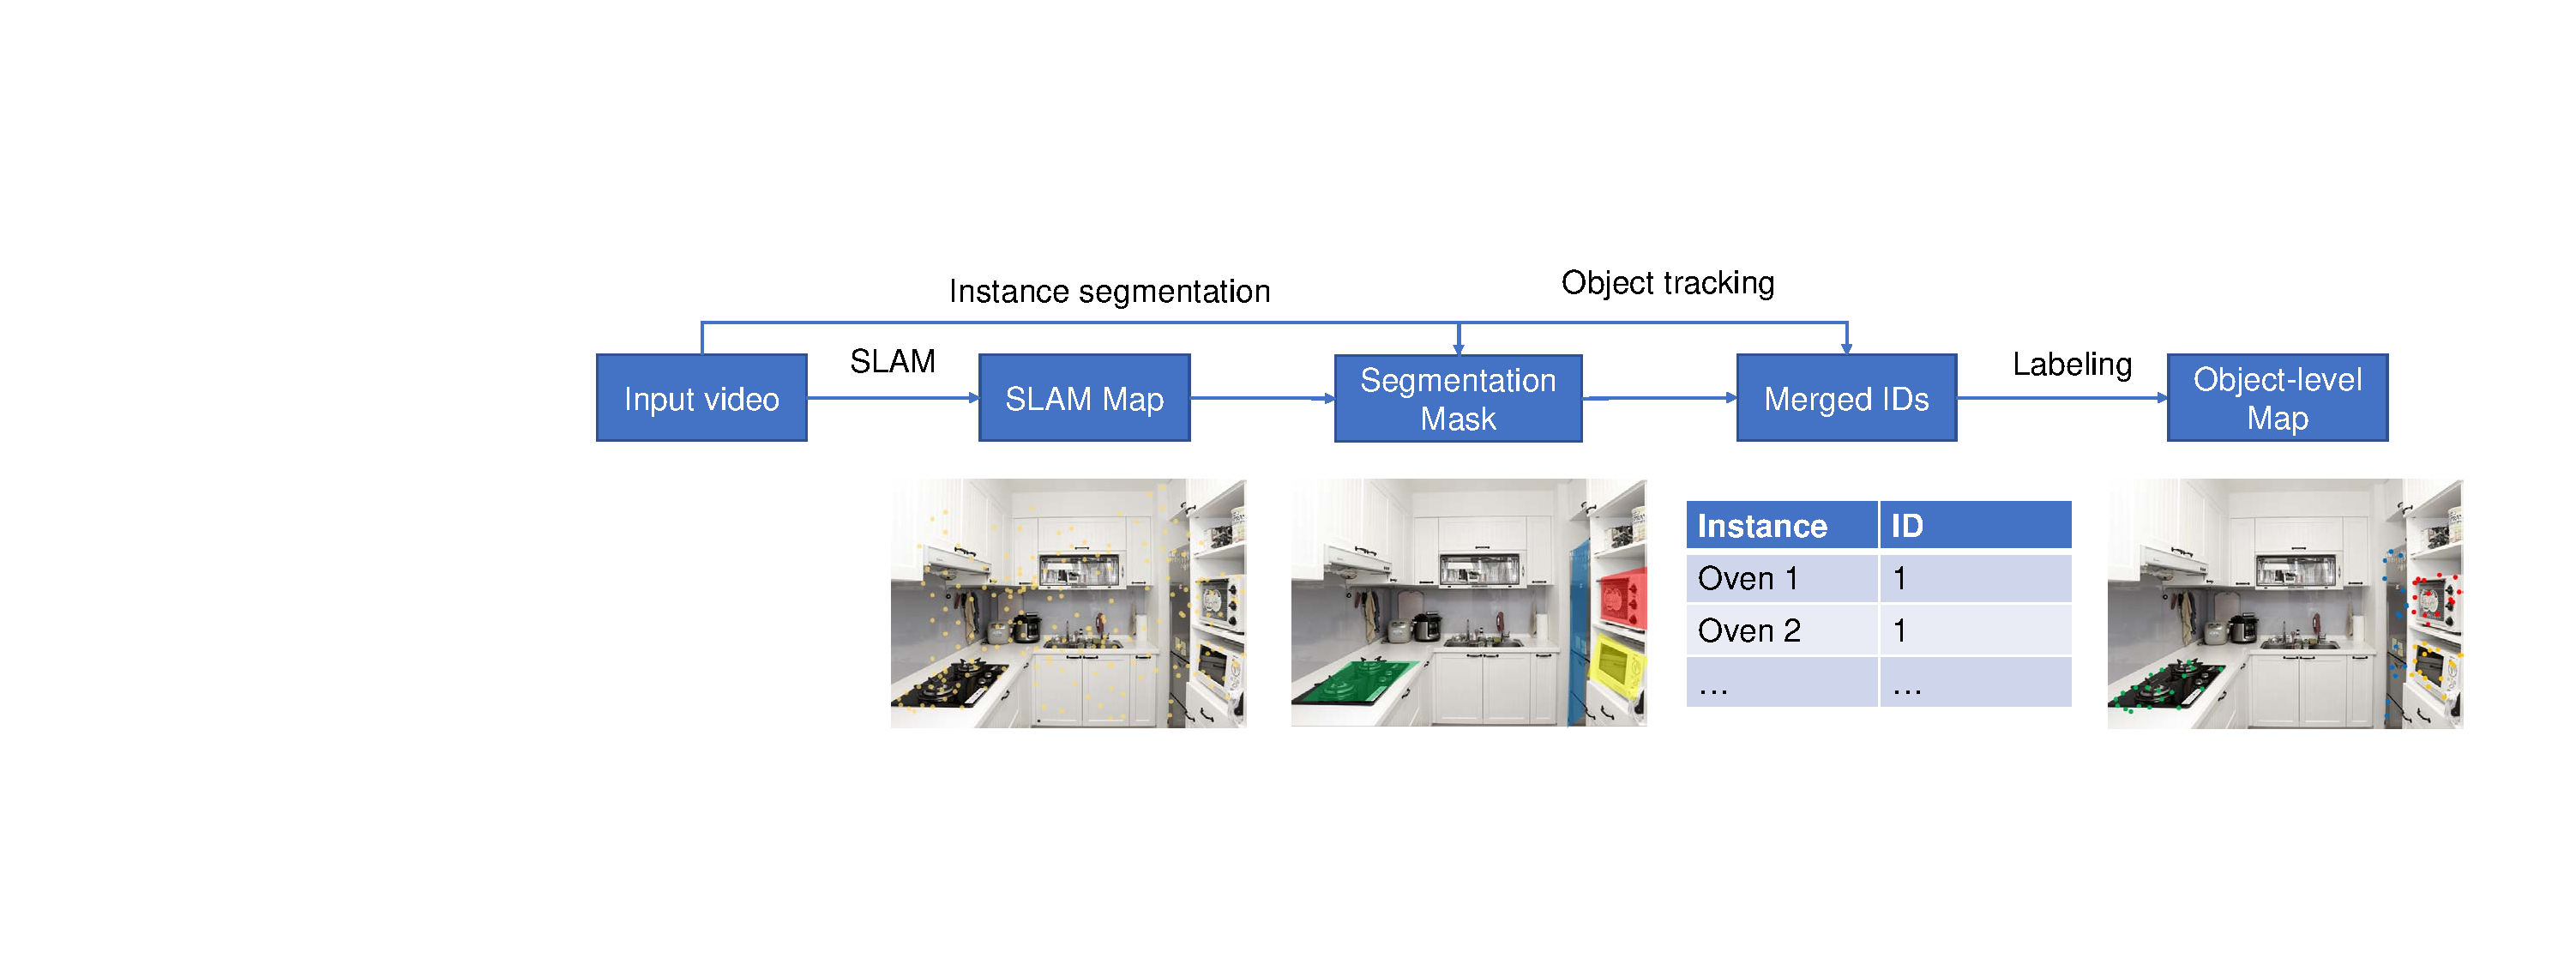
\includegraphics[width=0.99\linewidth]{offlinemap}
	\caption{对象级地图的构建过程}
	\label{fig:offlinemap}
\end{figure}

\subsection{对象级地图}\label{subsec:map}
为了实现基于VSLAM的对象识别,我们需要用相应的对象ID标记映射点。因此,我们称之为对象级映射。

最近,语义SLAM~\cite{bowman2017probabilistic,kaneko2018mask}和对象级SLAM~\cite{mccormac2018fusion++,strecke2019fusion}已被研究并显示出巨大的潜力。典型的用法是同时运行SLAM过程和语义分割神经网络,并使用分割结果来细化构建的地图。

\autoref{fig:offlinemap} 演示了构建对象级地图的工作流。
首先,我们将视频输入原始Visual SLAM进程~\cite{mur2017orb},并构建包含关键帧和贴图点的地图。
我们想要确定 1)环境中的哪些对象可以被视为交互目标,2)对于每个贴图点,它链接到哪个对象。
因此,我们使用实例分割神经网络\cite{He_2017_ICCV}来实现对输入视频的分割。对于每个检测到的对象,分割结果是像素级的二进制掩码$m$和对象类别$c$。
现在,我们在连续的帧中获得了很多对象,但它们还没有唯一地分配ID。为了防止潜在的重复检测,我们采用对象跟踪神经网络在不同的帧中合并相同的对象。
检测到的对象和贴图点之间的链接是像素坐标。
在SLAM过程中,当关键帧中的贴图点可见时,我们记录其像素坐标$(x,y)$,整个记录为$\{Index_m, Index_kf, (x,y)\}$。
对于每个关键帧的每个地图点,我们检查它们的坐标。如果坐标位于该关键帧的对象掩码内,则使用相应的对象ID标记地图点。

\subsection{地图长期重用}
在建立上述地图之后,我们可以使用该地图来识别稳定的对象。
如果稳定物体永远保持在同一位置,上述方法可以很好地工作。
然而,这在实践中很难实现。
如果稳定对象的位置与地图中记录的位置相比发生变化,我们希望主动检测此类变化并更新地图,从而使地图能够长期使用。

这里我们介绍计算2D-3D投影的RANSAC\cite{derpanis2010overview}算法,并观察移动的对象如何影响该算法。
选择具有类似BoW表示的候选关键帧后,RANSAC计算每个属于关键帧的$mp$和属于当前帧的$fp$之间的ORB特征相似性$s(ORB_{mp}, ORB_{fp})$。如果$s$低于某个阈值,$mp$和$fp$就会成功匹配,这意味着它们属于同一个物理点。
现在,RANSAC将随机选择$n$对匹配项,并通过PnP解算器计算投影$T$
\begin{equation}\label{equ:pnp}
    T = PnP([mp_1, fp_1],[mp_2, fp_2], ..., [mp_n, fp_n]).
\end{equation} 

然后,用$T$检查其余匹配点对,
\begin{equation}\label{equ:check}
    \
    err = T \cdot [mp_x, mp_y, mp_z] - [fp_x, fp_y],
\end{equation} 
其中下标$x,y$和$z$表示$mp/fp$的坐标。
当误差小于阈值时,这对点被视为一个内点,否则它是一个离群点。
在找到足够的内点后,$T$被视为正确的投影,并且将基于所有内点计算新的$T$。相反,如果没有找到足够的内点,RANSAC将从随机选取$n$对匹配项并从第一步开始重新启动。
因此,如果对象移动,潜在的结果可能是1)没有足够的内点进行定位,2)内点包含属于移动对象的地图点,从而导致错误的定位和识别。

我们修改了RANSAC算法,通过执行每个对象的投影来处理这样的对象移动。
在执行PnP解算器以计算$T$之前,我们根据地图点的对象标签对其进行聚类。
我们使用基于背景$T_{background}$的投影作为基准,因为背景通常是稳定的。
对于每个对象$O_i$,我们使用属于$O_i$的可见贴图点来验证$T$:

\begin{equation}\label{equ:gdt}
\
err = \Sigma \ T \cdot [mp_x, mp_y, mp_z] - [fp_x, fp_y].
\end{equation}
如果错误高于阈值,这意味着该对象的异常值太多,则我们确定该对象已移动。
详细的算法在算法\ref{alg::poa}中描述
可以通过投影粗略估计移动,因此我们仍然可以在正确的位置显示交互UI。
为了实现长期重用,我们需要根据\ref{subsec:map}节发送这些视频帧来更新地图。


\begin{figure}[t]
	\centering
	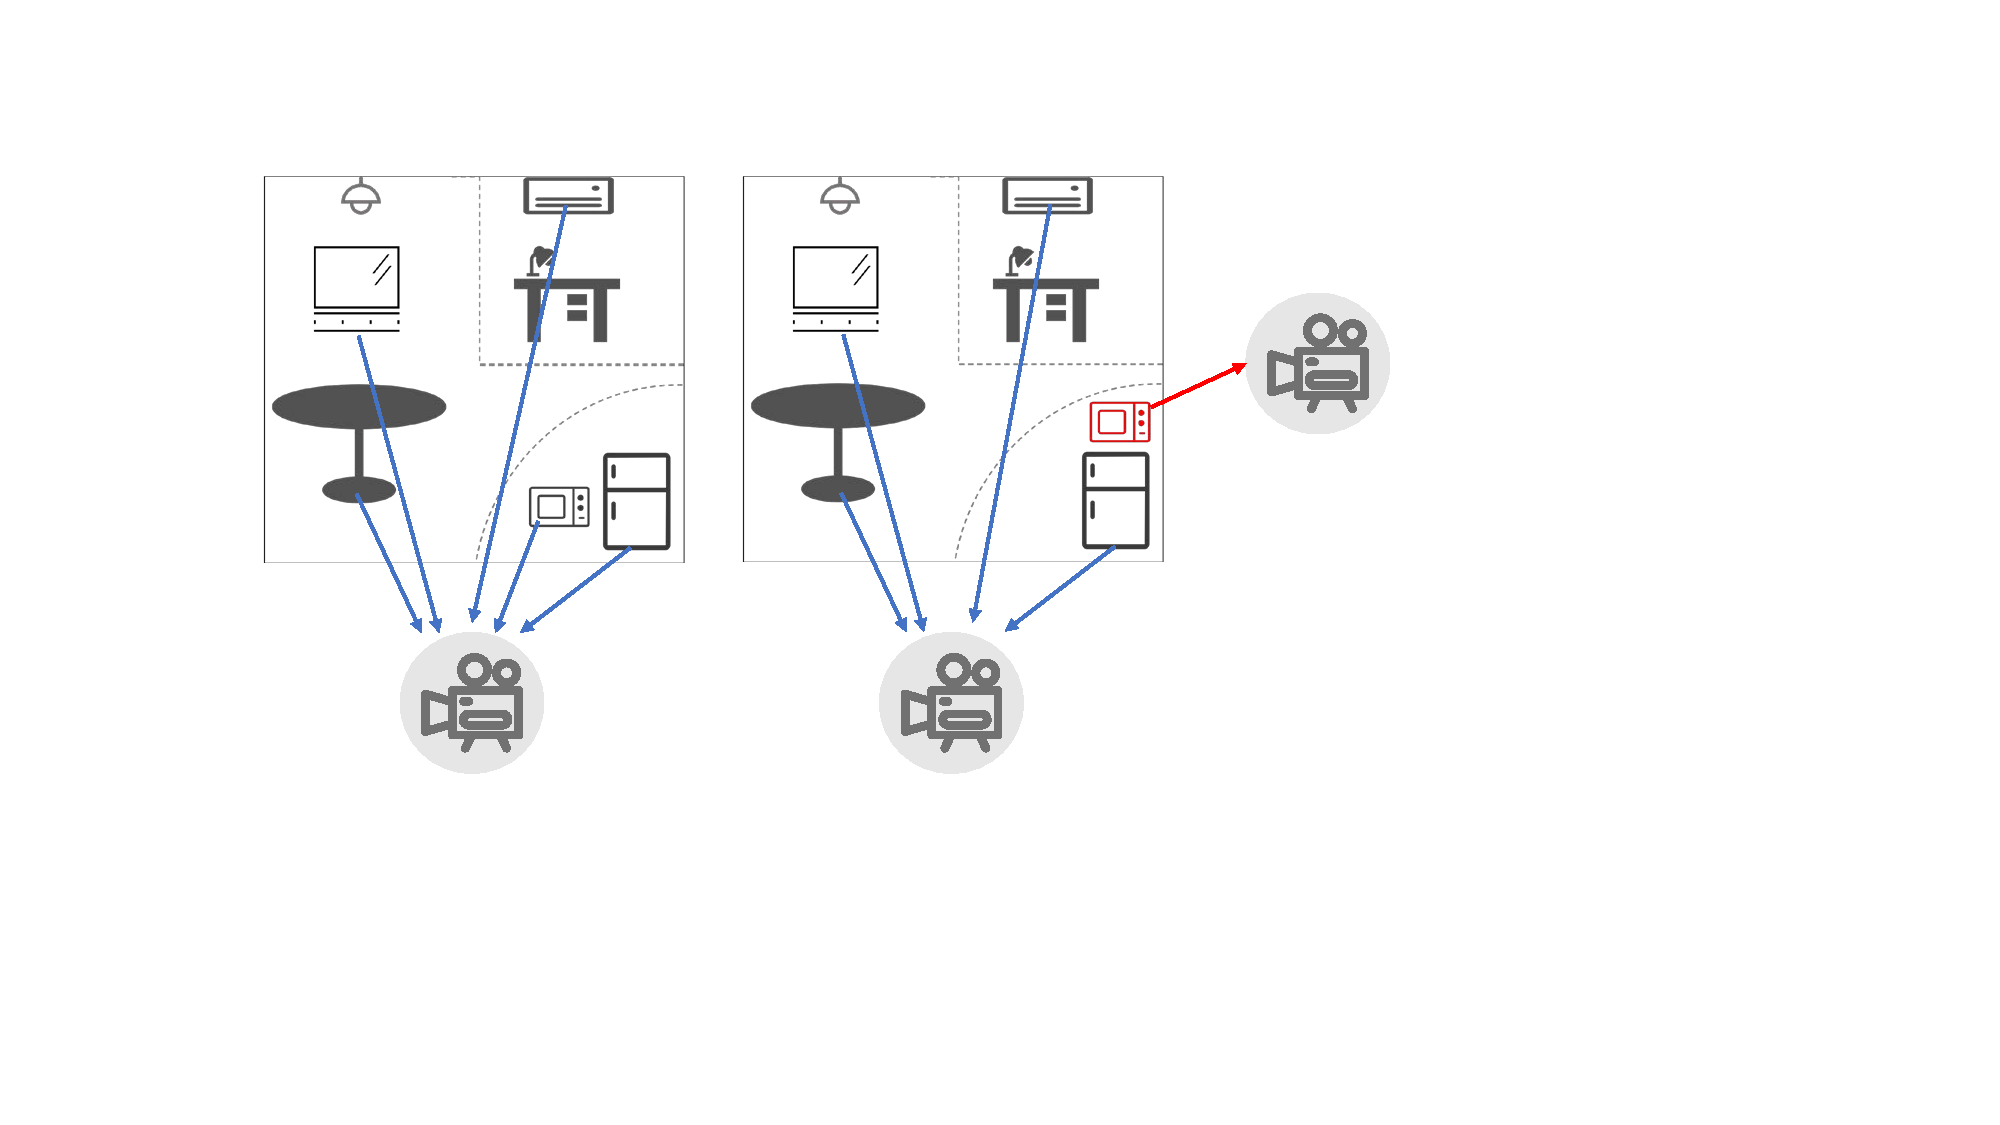
\includegraphics[width=0.7\linewidth]{moveobj}
	\caption{静态和动态目标的识别}
	\label{fig:move}
\end{figure}

\begin{algorithm}[t]  
	\caption{Per-Object-Projection }  
	\label{alg::poa}  
	\begin{algorithmic}[1]  
		\Require  
		$frame$: current video frame;
		$FPs$: feature points of $frame$;  
		$KFs$: keyframes of the map;  
		$MPs$: map points of the map;
		$OBJs$: q visible objects in $frame$;   
		\Ensure  
		camera pose $T_{cw}$;
		movement of $i_{th}$ object $OM_i$;
		\State initial $OM_i=0, i = 1,2,...,q$;
		\State initial $S_{mp}^i=\varnothing, i=1,2,...,q$;
		\State compute bag of words (bow) feature $bow_f$ for $frame$;
		\State Search $KFs$ for frames that share the same word with $bow_f$, then pick the most similar keyframe $KF_{candi}$;
		\For{each $mp\in KF_{candi}$}
		\For{each $fp\in frame$}
		compute the similarity $sim$ between $mp$ and $fp$;
		\If {if $sim < thre$}
		\State $S_{mp}^i = S_{mp}^i\cup\{(mp,fp)\}, i = mp_{label}$;
		\EndIf
		\EndFor 
		\EndFor
		\State compute camera pose $T_{cw}^{env} = PnPSolve(S_{mp}^i)$, $i$ corresponds to the ID of environment;
		\For{each $obj\in OBJs$}
		\For{each $mp\in S_{mp}^i$,  $i$ corresponds to $obj$ ID}
		\State compute camera pose $T_{cw}^{i} = PnPSolve(S_{mp}^i)$;
		\EndFor
		\EndFor
		\State compute and delete outlier in ${T_{cw}^{i}, i=1,2,...,q}$;
		\State recompute camera pose $T_{cw}$ with the left $S_{mp}^i$;
		\If {$T_{cw}^{i}$ is  outlier}
		\State $OM_i = Move_{cal}(T_{cw}^{i}, T_{cw})$; 
		\Else 
		\State {$OM_i = \vec 0$};
		\EndIf
	\end{algorithmic}
\end{algorithm}  

\begin{figure}[t]
	\centering
	\begin{subfigure}{.48\linewidth}
		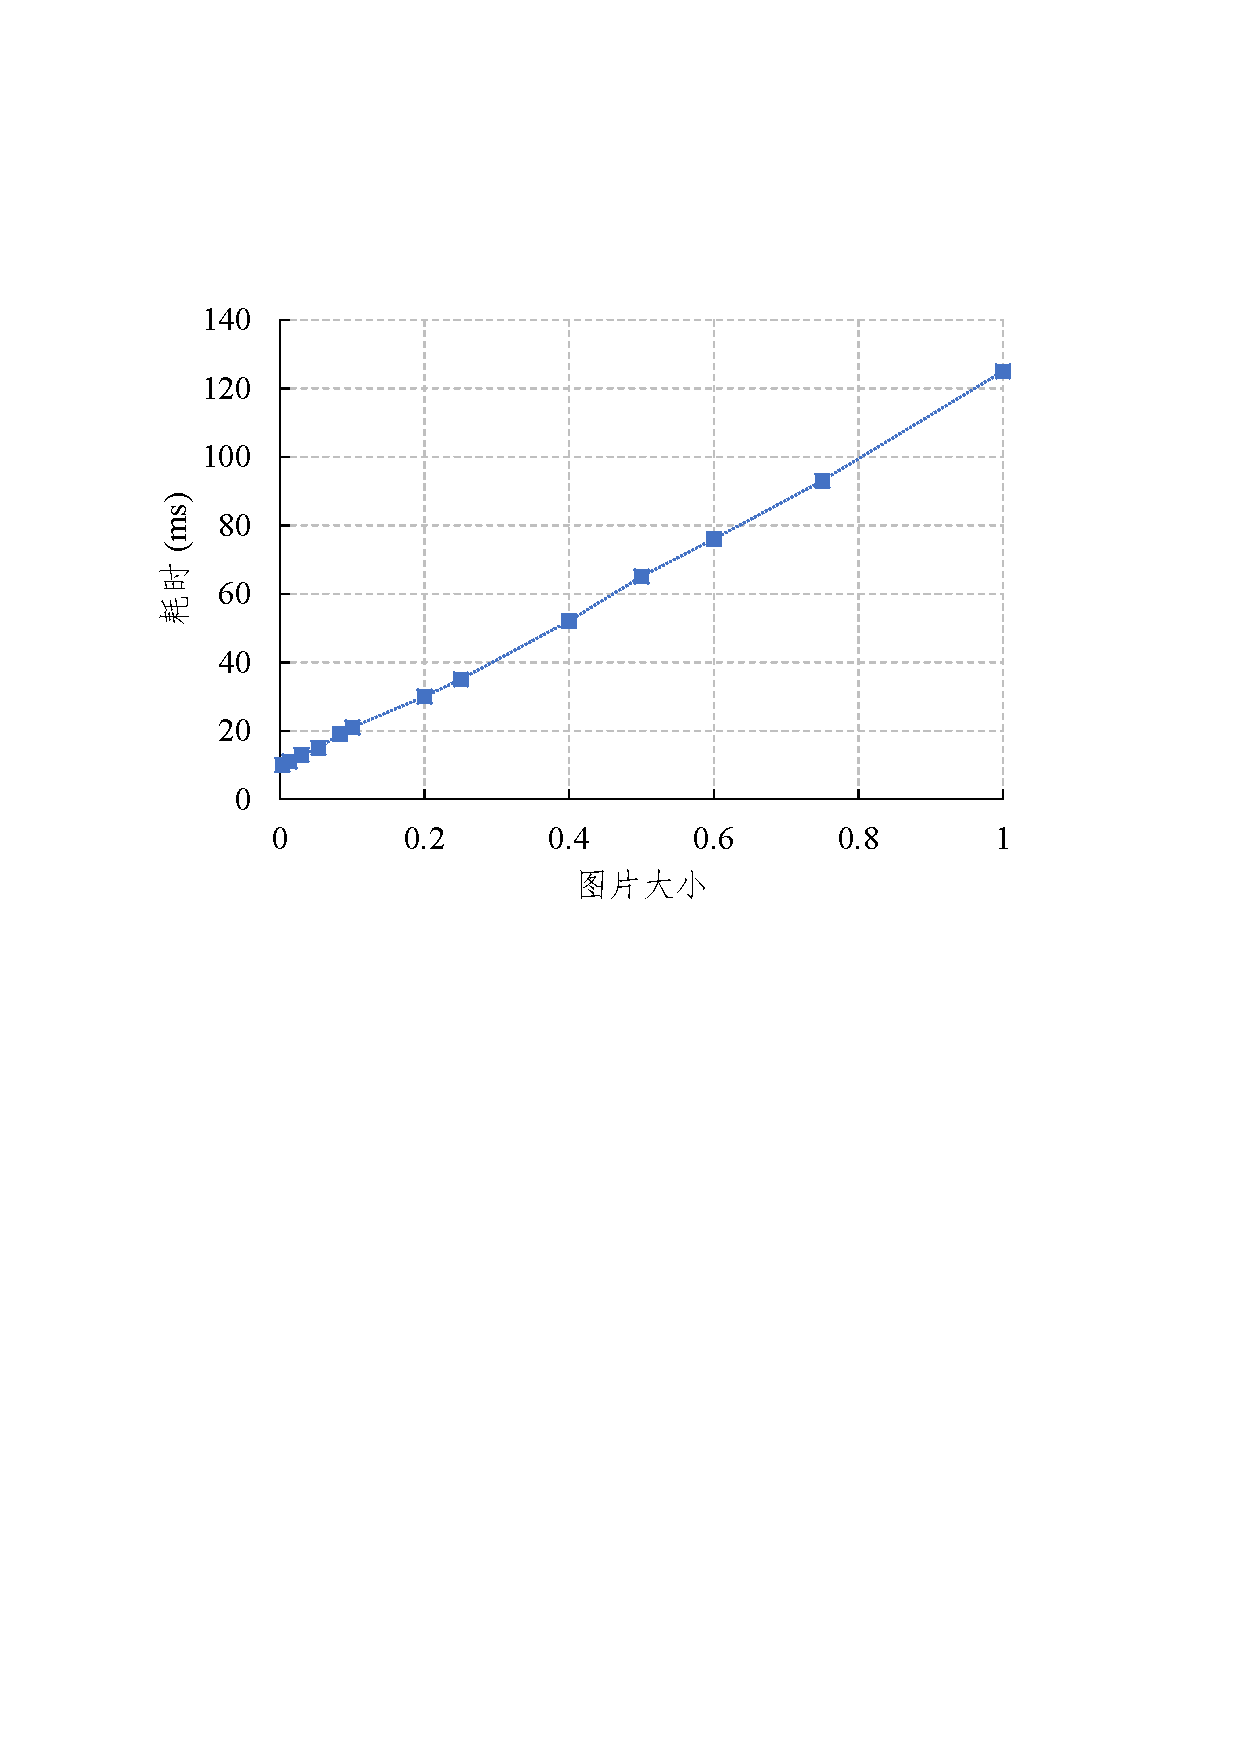
\includegraphics[width=1\linewidth]{static9}
		\caption{}
	\end{subfigure}
	\ 
	%\hskip2em\
	%\centering
	\begin{subfigure}{.48\linewidth}
		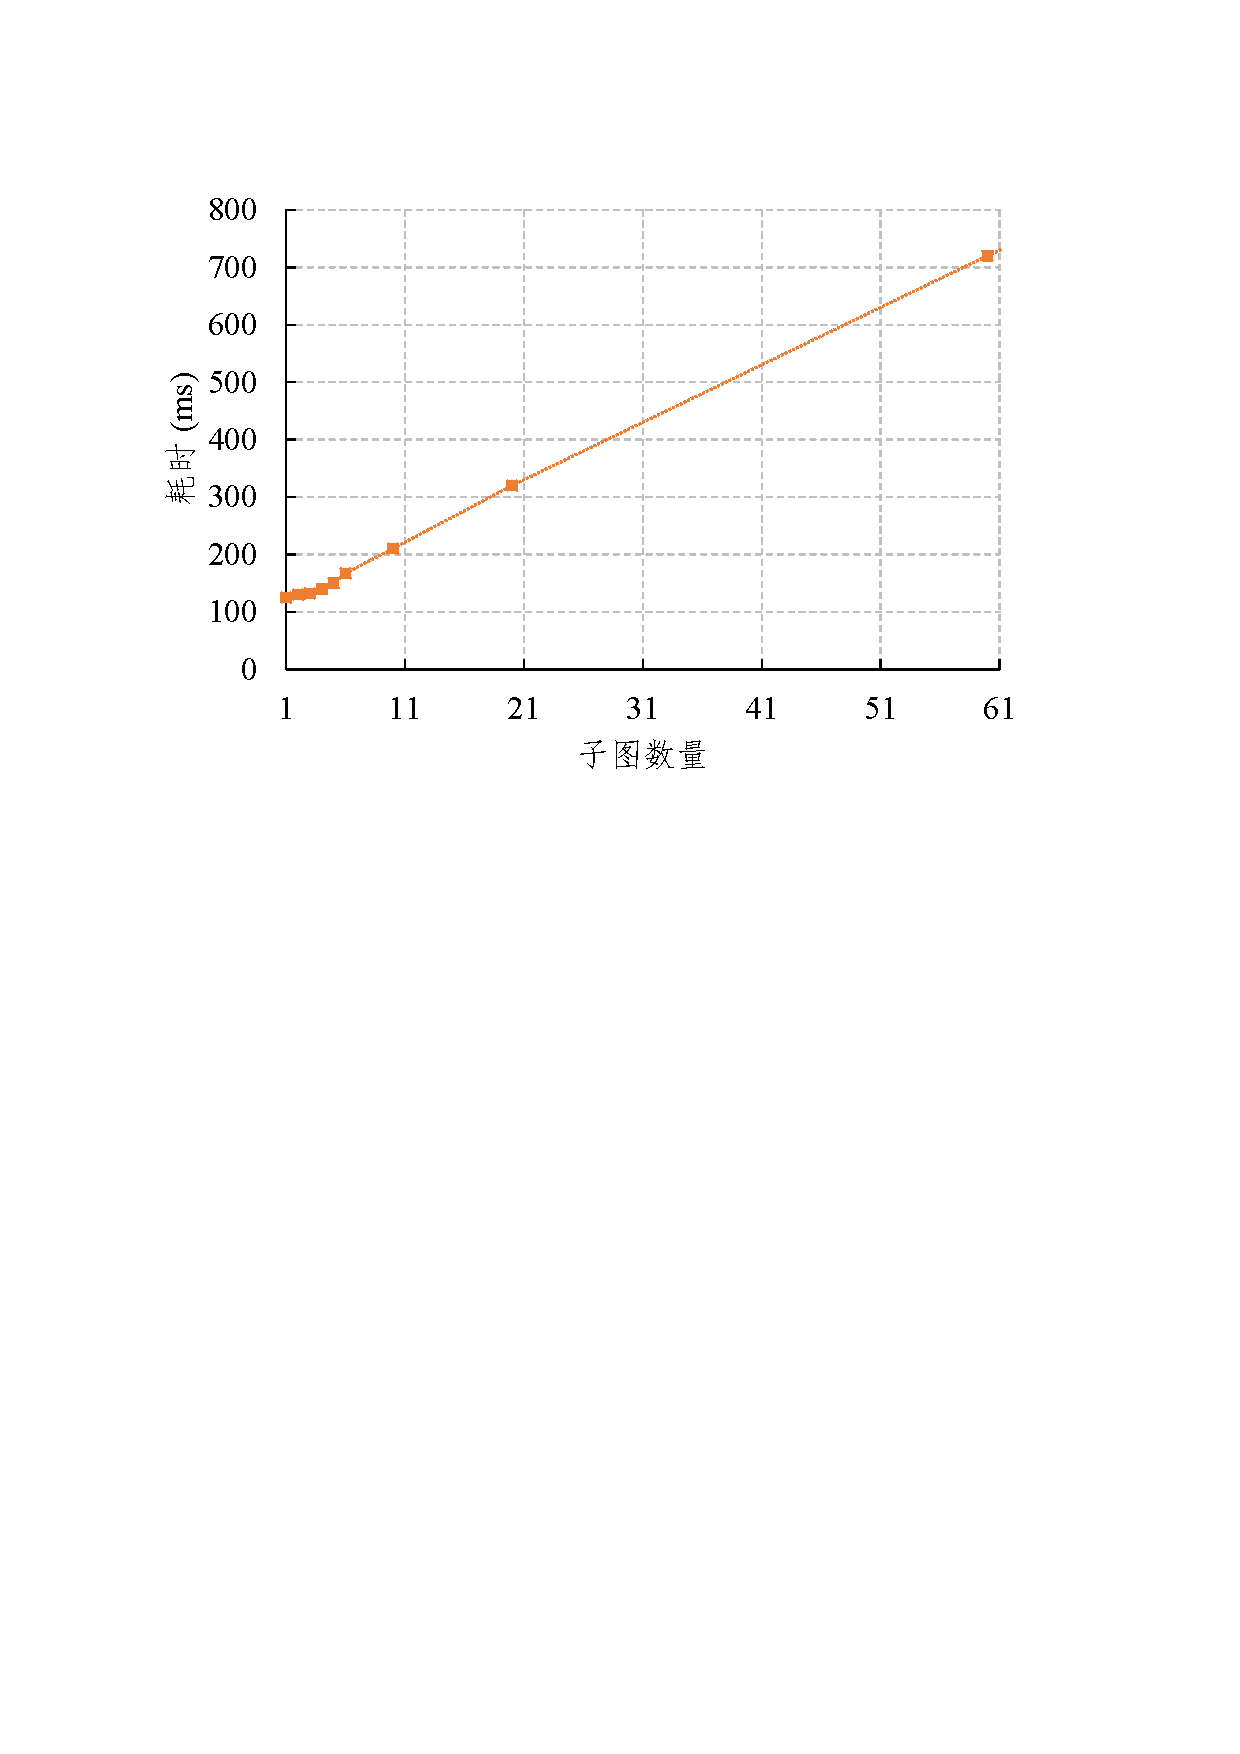
\includegraphics[width=1\linewidth]{static10}
		\caption{}
	\end{subfigure}
	\caption{子图的神经网络推理时间花费}\label{fig:subframetime}
\end{figure}


\begin{figure}[t]
	\centering
	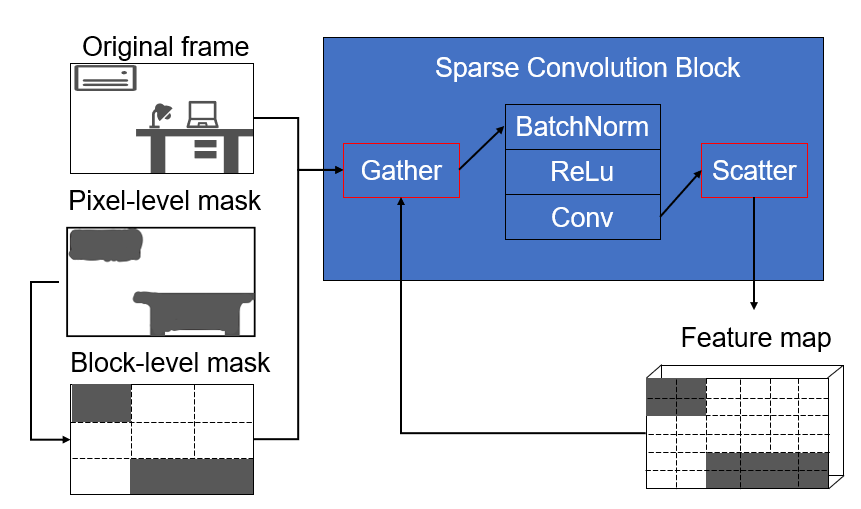
\includegraphics[width=0.75\linewidth]{temp}
	\caption{我们提出的推理加速方法工作流程}
	\label{fig:sparse-conv}
\end{figure}


\subsection{基于稀疏推理的网络加速}\label{sub:Sparse Object Detection}
在\ref{subsec:vslam}节里我们描述了如何利用Visual SLAM和构建的对象级映射来识别稳定对象。然而,我们仍然无法识别会发生位置改变的物体。

如\ref{subsec:motivation}节所说,目标识别网络和图像检索可以用于移动物体的识别。目标识别神经网络首先在被检测的物体上产生一个二维的包围盒,然后可以使用图像检索技术在数据库中找到它所对应的ID。

然而这种实现收到神经网络计算时间的限制。尽管研究者们已经在努力通过网络压缩和轻量设计等方式尝试缩短神经网络推理的时间,但在手机上或者只具备CPU的边缘设备上实现实时仍然很难做到。


\subsubsection{检测先验}
% vslam的结果可以产生prior
% mask的产生可以使用前面建图的mask
% 直接依据先验来切分图片的做法结果不好 

我们通过输入约简的方式加快网络推理的速度。
如\ref{subsec:vslam}节所述,Visual SLAM可以检测稳定的对象。因此,神经网络不需要对属于稳定对象的区域进行计算。

我们考虑了用于确定检测优先级的不同方法,即如何确定神经网络应忽略的特定区域。
我们可以使用属于某个稳定对象的地图点集作为先验知识来形成该区域。
然而,这种方法提供的先验知识并不完整。
原因是检测到的地图点没有最佳分布。
在Visual SLAM定位过程中,只有一部分特征点(当前帧中)可以投影到地图点(地图中),并且分布是随机的。
假设我们检测到$N$特征点属于一台电视机,则$N$特征点可能都集中在电视机的一个角落。
不完整的先验使得神经网络必须分析更多的区域,这意味着无法获得更多加速。
为了获得精确完整的先验知识,我们在\ref{subsec:map}节中重用实例分割神经网络生成的对象掩码。检测先验可通过以下公式计算:
\begin{equation}\label{equ:mask}
mask_c^i = Trans(Pose_c,Pose_k)mask_k^i.
\end{equation} 

$mask_c^i$表示当前帧中对象$i$的二进制掩码,这是我们的前一帧$mask_k^i$是对象$i$最相关关键帧中的二进制掩码。$Trans(Pose_c,Pose_k)$计算了当前帧和关键帧之间的摄影机姿势变换。

利用检测先验知识,一种直接的减少输入的方法是将原始帧划分为多个子帧,然后分别对其进行推断。
然而,实验表明,这种实现通常比处理原始帧需要更多的时间。
原因是这种“分而治之”的实现降低了计算的并行性。我们需要在for循环中处理这些子帧。此外,许多小尺寸的子帧无法从现有的GEMM优化方法中获益。

从\autoref{fig:subframetime}a中,我们使用$640\times 480$的帧作为标准的图片大小1,图片的大小体现在X轴,我们在不同大小的帧上使用相同的神经网络进行测试,我们可以看到帧的大小$s$和推断时间$t$的关系为$t = as + b, a>0,b >0$,这意味着神经网络推理有一个固定的时间成本,哪怕帧的大小为1个像素点。在我们的测试中,$b$为11毫秒。
\autoref{fig:subframetime}b中,我们将原本的一帧划分成多个子图,测试的结果显示,当我们将帧划分为越来越多的子图时,总的时间开销不断增加。
 
\subsubsection{\textbf{稀疏推理}}
稀疏卷积\cite{graham2015sparse,ren2018sbnet}可以利用输入的稀疏性来减少延迟。
在VSLink中,我们遵循\cite{ren2018sbnet}的思想设计了具有稀疏块的目标检测神经网络。

这种稀疏卷积设计~\cite{ren2018sbnet}的关键思想是引入聚集/分散核来实现张量形状变换。
基本工作流程如下所示。

首先,我们使用$h\times w$矩形覆盖原始的像素级二进制掩码,该掩码生成一个新的块级掩码。
然后,原始的4-d$N \times H \times W \times C$帧和2d$H/h \times W/w$掩码被发送到卷积块。给定掩码中设置为1的$B$块,散射(scatter)随后使用$h\times w \times C$切片将块从输入张量中切片,并将B切片沿batch的维度堆叠到新张量中,生成$B\times h \times w \times C$张量。
在收集之后,可以将张量发送到正常的卷积块。
在卷积计算之后,需要对结果进行整形以形成特征映射,该特征映射由散射核实现。
散射过程是反演收集,我们根据二元掩模将卷积结果的$h\times w \times C$切片提取到特征图中。整个推理加速图如\autoref{fig:sparse-conv}所示,图中特征图引出的箭头表示下一层会重复类似的计算过程。


\subsubsection{\textbf{识别和追踪}}
如果一个物体被神经网络检测到,我们通过图像检索来识别它的物体ID。检索基于深度卷积特征。
在构建\ref{subsec:map}节所述地图的过程中,我们使用与目标检测神经网络相同的骨干网络提取并保存检测到的可移动目标的深度卷积特征。
在图像检索过程中,对于每个检测到的对象,我们将其特征与数据库中存储的特征进行比较。如果特征相似性达到一个阈值,我们就可以认为识别到了对象。
运动目标的跟踪是通过特征点跟踪来实现的,与稳定目标的跟踪类似。
只要特征点在连续的帧中可见,我们就临时跟踪属于某个可移动对象的特征点。

\begin{table}[t]
	\centering
	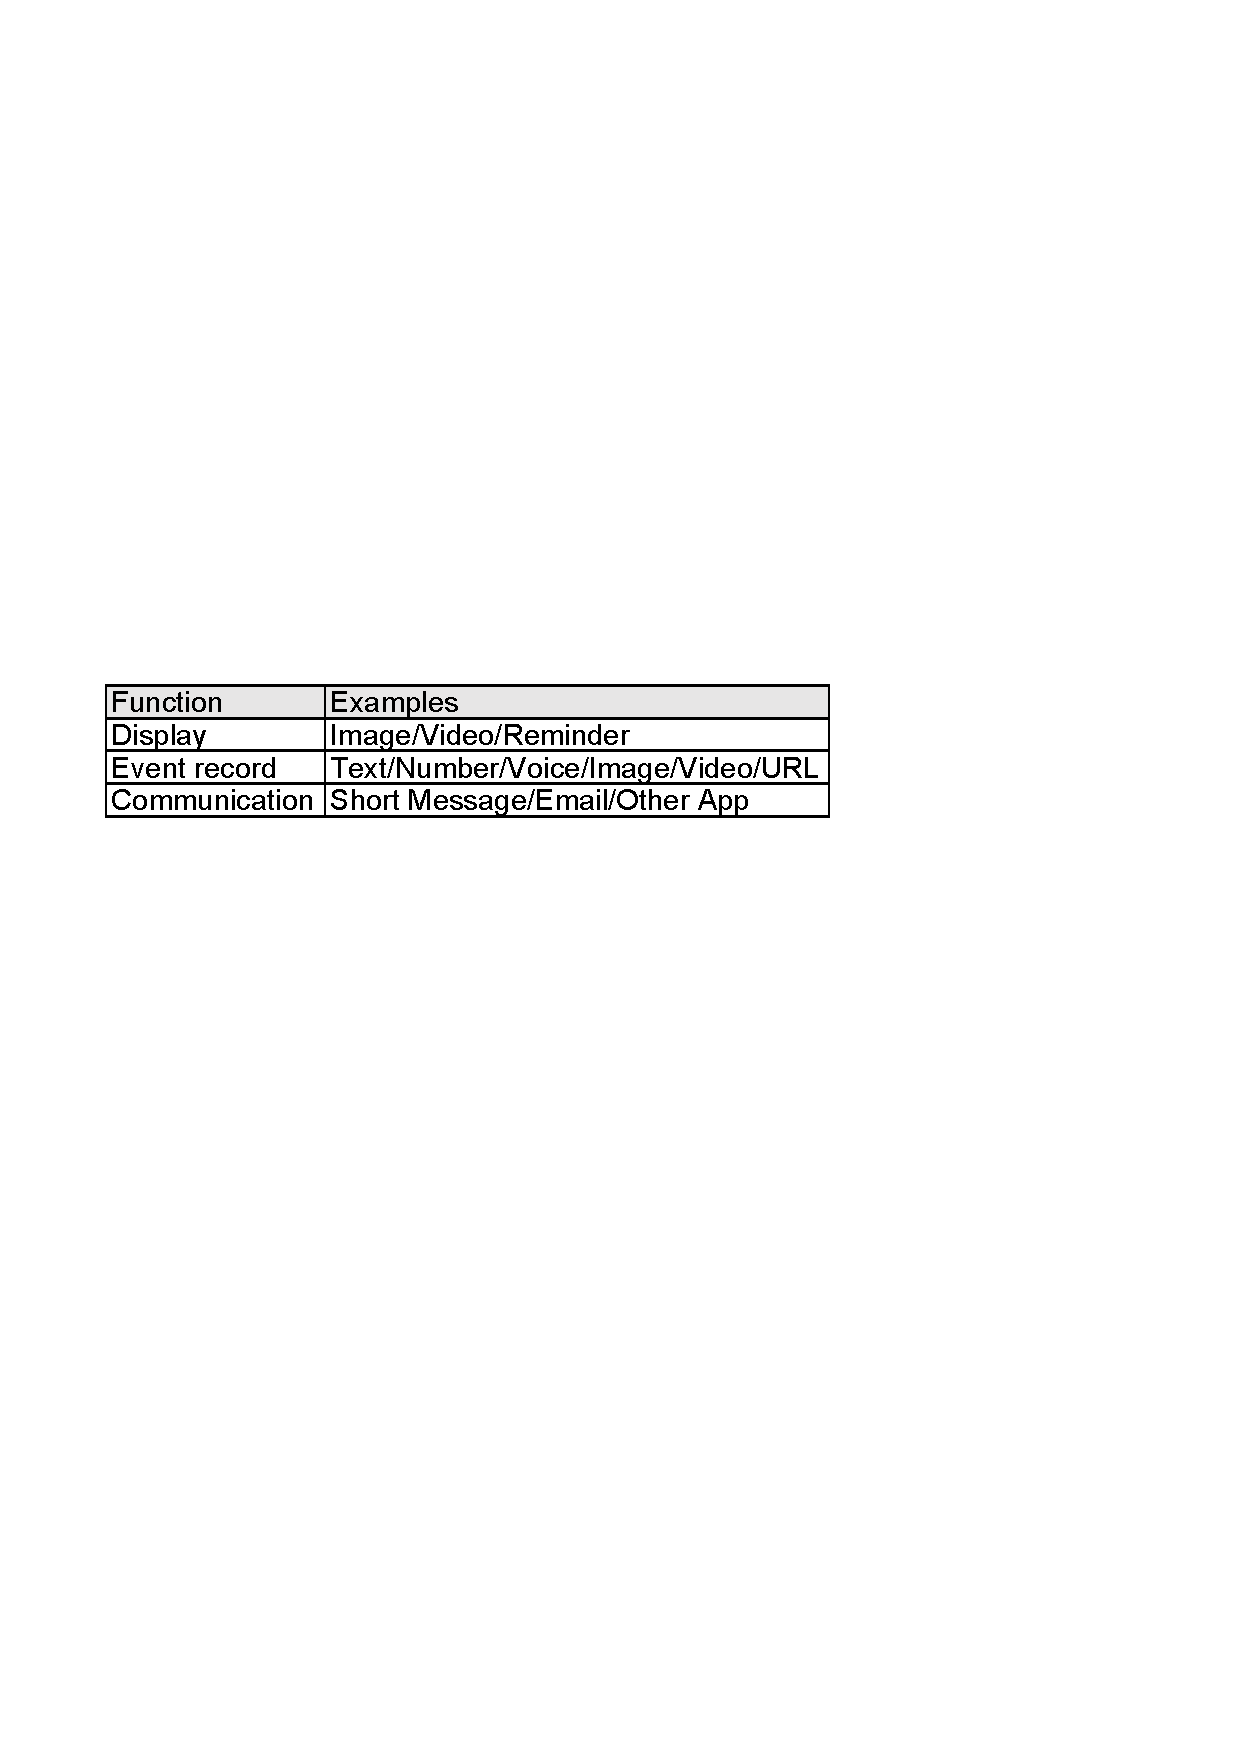
\includegraphics[width=0.98\linewidth]{functions}
	\caption{VSLink在不可连接对象上实现的功能}
	\label{table:functions}
\end{table}

\section{定制化交互}\label{sec:flexible}
VSLink旨在丰富人与对象之间的交互。
大多数现有的人机交互实现都遵循一个由程序员决定一切的过程,比如交互目标、功能和UI。
如\ref{sec:introduction}节中所述,VSLink通过合并不可连接的对象扩展了交互目标的概念,这意味着用户可以自由确定对象是否为交互目标。
我们希望保留让用户决定交互的设计理念。
\subsection{功能抽象}
为了实现与不同对象的交互,VSLink需要实现相应的UI。
然而,为每个可能的对象设计完整的UI,包括功能和外观,实际上是无法做到的。
即使对象属于同一类别,功能稍有不同也会使得交互方式发生细微改变。
例如,与普通灯相比,智能LED灯具有更多的功能,例如颜色和亮度调整。
因此,VSLink提取和抽象对象的\textit{最小功能单元},并基于这种抽象设计UI。
对于可连接对象,制造商已经定义了最小功能单元,我们只需要遵循其接口。
考虑到不可连接的对象没有预定义的接口,我们提出了三种类型的函数来实现交互。
这些功能基于手机的交互方式,我们认为这有助于人机交互。

% Event Recording
% Communication
% Information Display
% 
 
\subsection{面向用户的UI设计}
通过获取一组最小的功能单元,用户可以根据个人需要设计完整的用户界面。
VSLink使用基于web的UI设计框架,用户可以在其中调整对象UI的外观、布局和逻辑。
整个设计过程没有代码,只需要拖放操作。
为了减少用户在设计UI时的负担,我们鼓励用户从UI模板开始自己的设计。
我们提供多个具有代表性的用户界面模板。根据对象类别,建议用户选择某个模板,开始定制UI设计。

\section{实现和验证}\label{sec:eval}
\subsection{实现}
\textbf{软件}: 我们基于ORB-SLAM2~\cite{mur2017orb}实现了两阶段目标识别模块的Visual LSAM部分,该模块得到了广泛的应用和评估。我们继承了它用于地图构建和跟踪的代码,并开发了地图点标记、对象识别和逐对象投影的代码。
我们在VSLink中采用了SOTA轻量级目标检测模型yolov5s~\cite{glenn_jocher_2020_4154370},因为它在速度和精度上具备优越性。我们修改了网络,使其支持稀疏卷积~\cite{ren2018sbnet}。
我们通过LibTorch使得神经网络在C++环境中执行。
对于图像检索,我们使用目标检测神经网络最后一个特征提取层的输出~\cite{glenn_jocher_2020_4154370}作为特征表示。两阶段目标识别模块的所有代码都是用C++编写的。

我们为用户实现了一个基于web的平台,用户可以在其中设计定制的交互。
在前端有基本单元(用于最小功能单元的UI)和画布。
通常,用户可以通过将基本单元拖动到画布来实现自己的设计。
我们还为不同的对象准备了多个UI模板,这可以简化设计过程。
这个平台的代码是用HTML5编写的。

\textbf{硬件}: 我们采用了智能手机Oneplus 7作为移动AR设备,它有一个骁龙855处理器和8GB的RAM。边缘服务端使用一台带有ubuntu系统的PC,它有16G的RAM和一个8核CPU。
\subsection{实验设置}

我们在真实的校园实验室环境中评估了VSLink。为了收集视频数据,我们在5天内对实验室进行了5次录像。
第一次的视频长度为8分钟,该视频用于构建对象级地图。其余视频的长度为3分钟,用于评估。在第四次和第五次,我们手动更改六个对象的位置。

\subsection{评估}

\begin{table}  
	\small  
	\caption{各类对象所提取的特征点数量(部分)}  
	\begin{center}  
		\begin{tabular}{|l|l|l|l| p{4cm}|}  
			\hline  
			\textbf{Filtered} & \textbf{MPs} & \textbf{Reserved objs} & \textbf{MPs}\\ \hline  
			box & 15 & PC & 355  \\ \hline 
			chair & 13 & table & 239  \\ \hline 
			chair & 9 & display & 83  \\ \hline  
			chair & 22 & Paper cutter & 226  \\ \hline  
			box & 43 & printer & 291  \\ \hline  
			chair & 9 & water fountain & 216  \\ \hline  
		\end{tabular}  
	\end{center}  
\end{table}\label{table:mps}  

\textbf{地图构建} 
在为环境构建地图的过程中,我们首先过滤绑定到非常少地图点的对象。
这是因为地图点的数量直接影响识别性能。在\autoref{table:mps}中我们列出了保留和过滤的对象,我们可以看到过滤后的对象通常尺寸较小或没有丰富的视觉特征,这符合ORB-SLAM2\cite{mur2017orb}的地图点选择方法的原则。
最后,我们选择了20个对象作为交互目标,包括13个可连接对象和7个不可连接对象。

\begin{figure}[t]
	\centering
	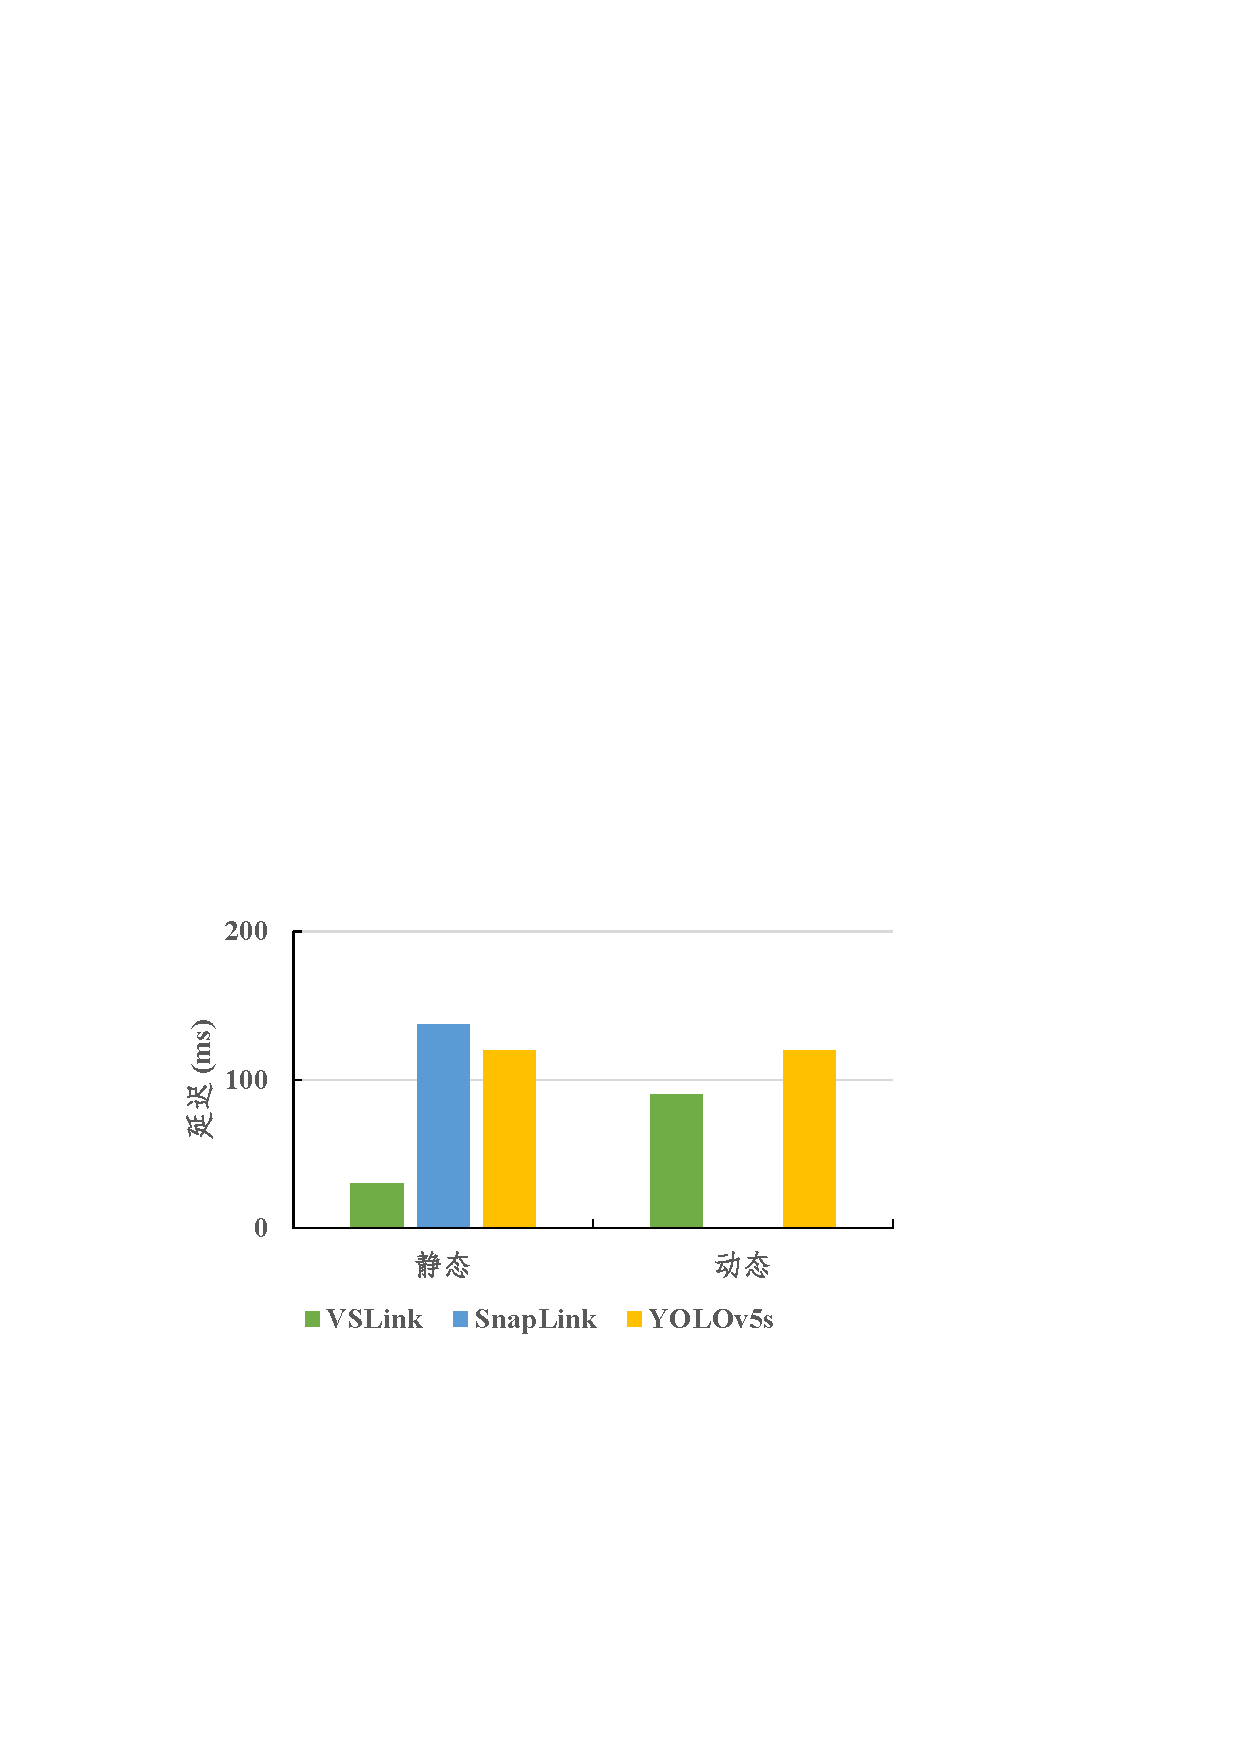
\includegraphics[width=0.65\linewidth]{latency_all.pdf}
	\caption{系统延迟对比}
	\label{fig:latency comparison}
\end{figure}

\textbf{System latency}: 
我们将对象识别的VSLink延迟度量与其他方法进行了比较。考虑了两种方法。一种是SnapLink\cite{chen2018snaplink}采用的基于图像定位的方法,另一种是将目标检测神经网络与图像检索相结合。我们用于比较的神经网络是原始的YOLOv5s\cite{glenn_jocher_2020_4154370},没有稀疏卷积修改。

我们在同一台机器上对四个视频运行了20次这些算法,结果显示在\autoref{fig:latency comparison}中。
首先,我们可以看到,对于那些稳定的对象,VSLink可以在20毫秒内检测到它们的存在,这与ORBSLAM的运行频率一致。在这个过程中,VSLink不需要计算视觉特征,而是重用SLAM结果。
然而,其他两种方法需要更多的时间进行特征计算,即100ms以上。
然后,对于可移动对象,SnapLink无法处理这种情况,因为场景与数据库中的图像不匹配,而对于神经网络,其花费的时间与稳定对象相同,大于100ms。
VSLink平均需要76毫秒左右才能完成加速推理。然而,这不是每个帧都需要的,因为\cite{yao2020video}已经提出了基于帧变化选择性执行对象检测的方法。
因此,VSLink的整个平均处理时间在33ms以下。
虽然原始的YOLOv5s方法不需要等待其他过程,但它完成推断需要120毫秒。
 
总而言之,VSLink可以支持每秒30帧的视频流,用于多对象识别,并且在速度上优于其他两种方法$4$倍。

\begin{figure}[t]
	\centering
	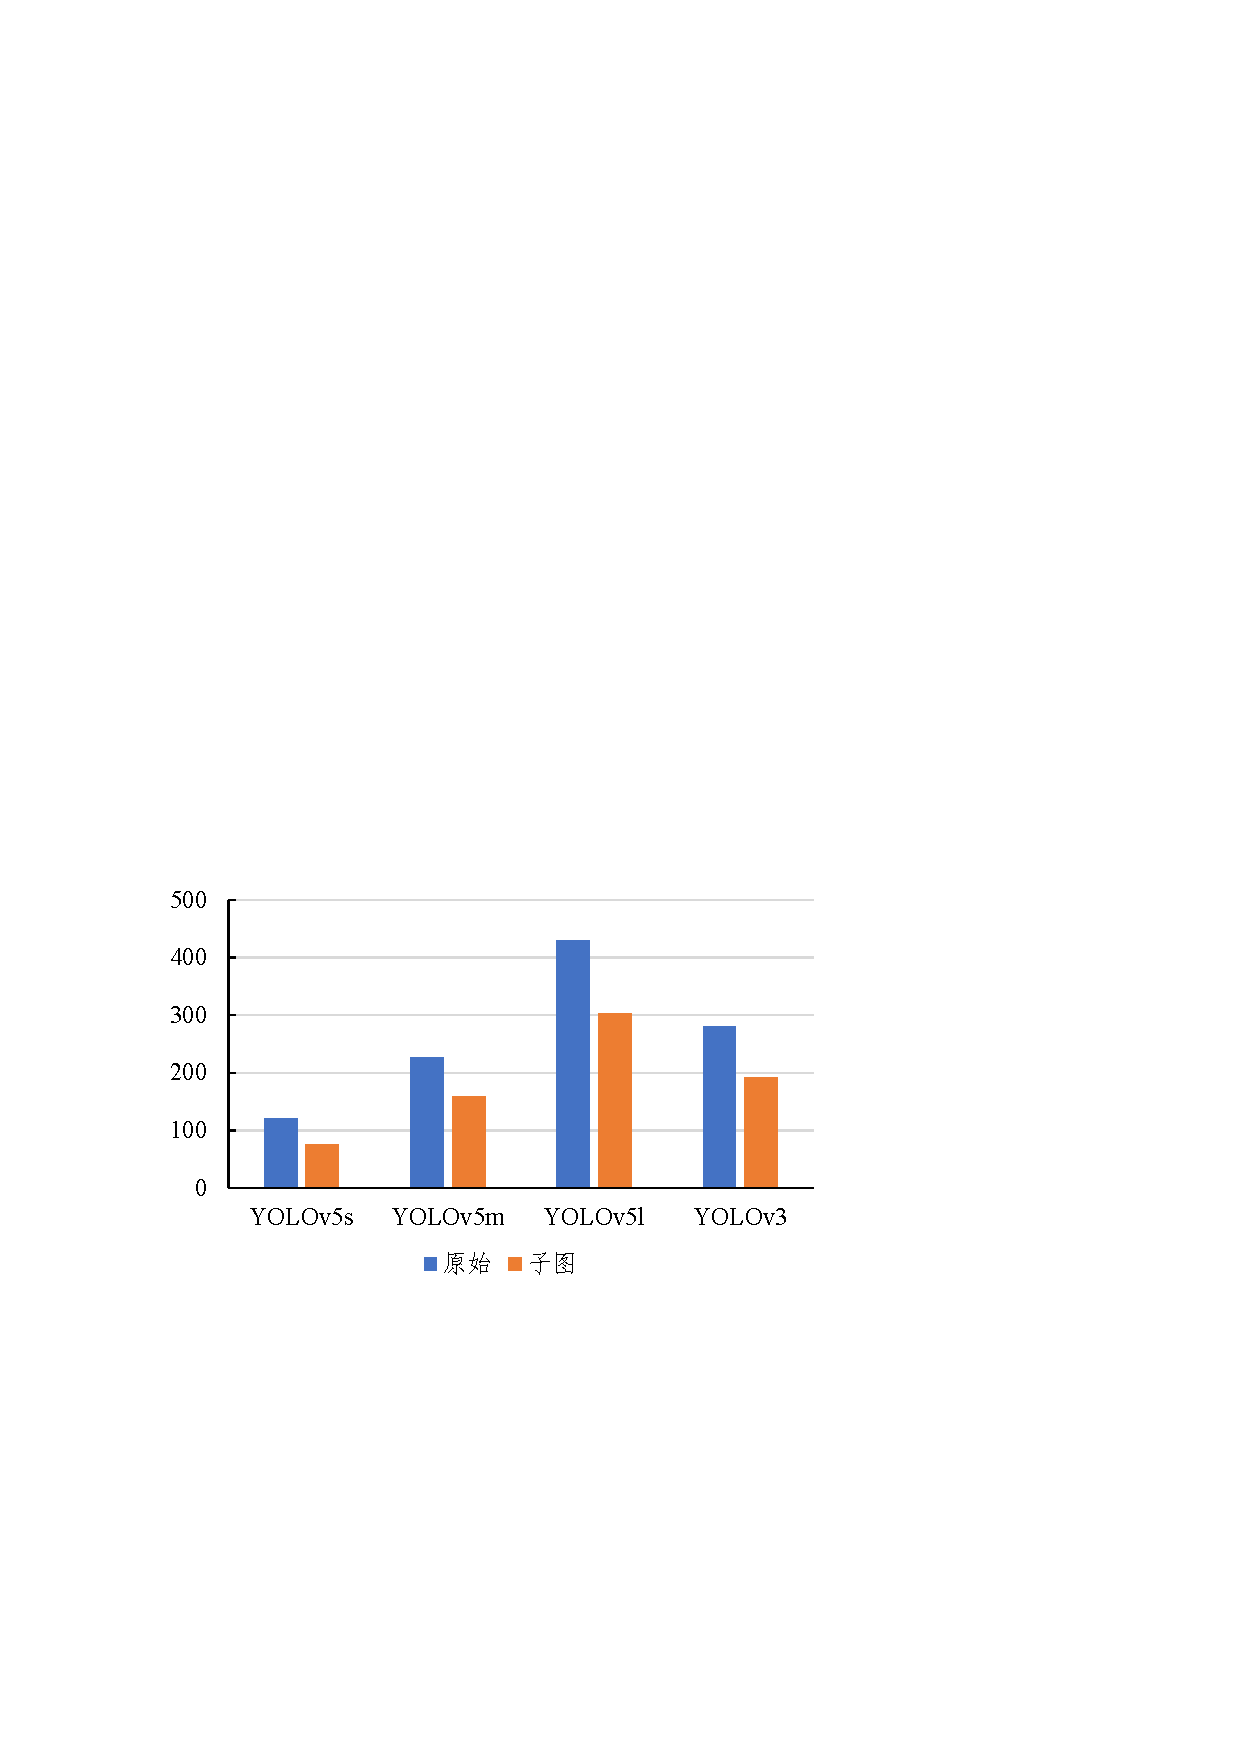
\includegraphics[width=0.65\linewidth]{NN1.pdf}
	\caption{使用子图后目标检测延迟的改善}
	\label{fig:latency improvement}
\end{figure}

\textbf{稀疏推理加速}:
我们采用高性能的目标检测神经网络YOLO\cite{redmon2016you}来评估我们提出的推理加速方法。
我们选择了不同尺寸和结构的模型,分别为YOLOv5s、YOLOv5m、YOLOv5l和YOLOv3,其中s、m、l表示模型尺寸。
所有神经网络都在Pytorch中训练,并使用TorchScript导出。导出之后,可以在C++环境中调用它们。
在\autoref{fig:latency improvement}中,我们通过引入检测先验和稀疏卷积来显示神经网络的延迟减少。这表明所有的神经网络都有延迟下降。YOLOv5s、YOLOv5m和YOLOv5L的速度提升分别为33.1\%、34.4\%和37.0\%。
我们认为更大的模型会得到更好的速度提升。

在实验中,我们对YOLO系列模型进行了测试。
然而,这只是目标检测神经网络的一种类型。
我们认为,只要网络中包含卷积块,理论上所有的目标检测神经网络都将受益于这种推理加速。对于其他类型的神经网络,加速程度将有所不同。
例如,已知更快的RCNN是精确的两阶段模型,加速的过程不同于一阶段模型。
对于两阶段模型,将首先使用RPN生成包围盒,然后使用分类模型生成对象标签。由于涉及到完全连接层,我们需要在一阶段之后进行计算修改。


\begin{figure*}[t]
	\centering
	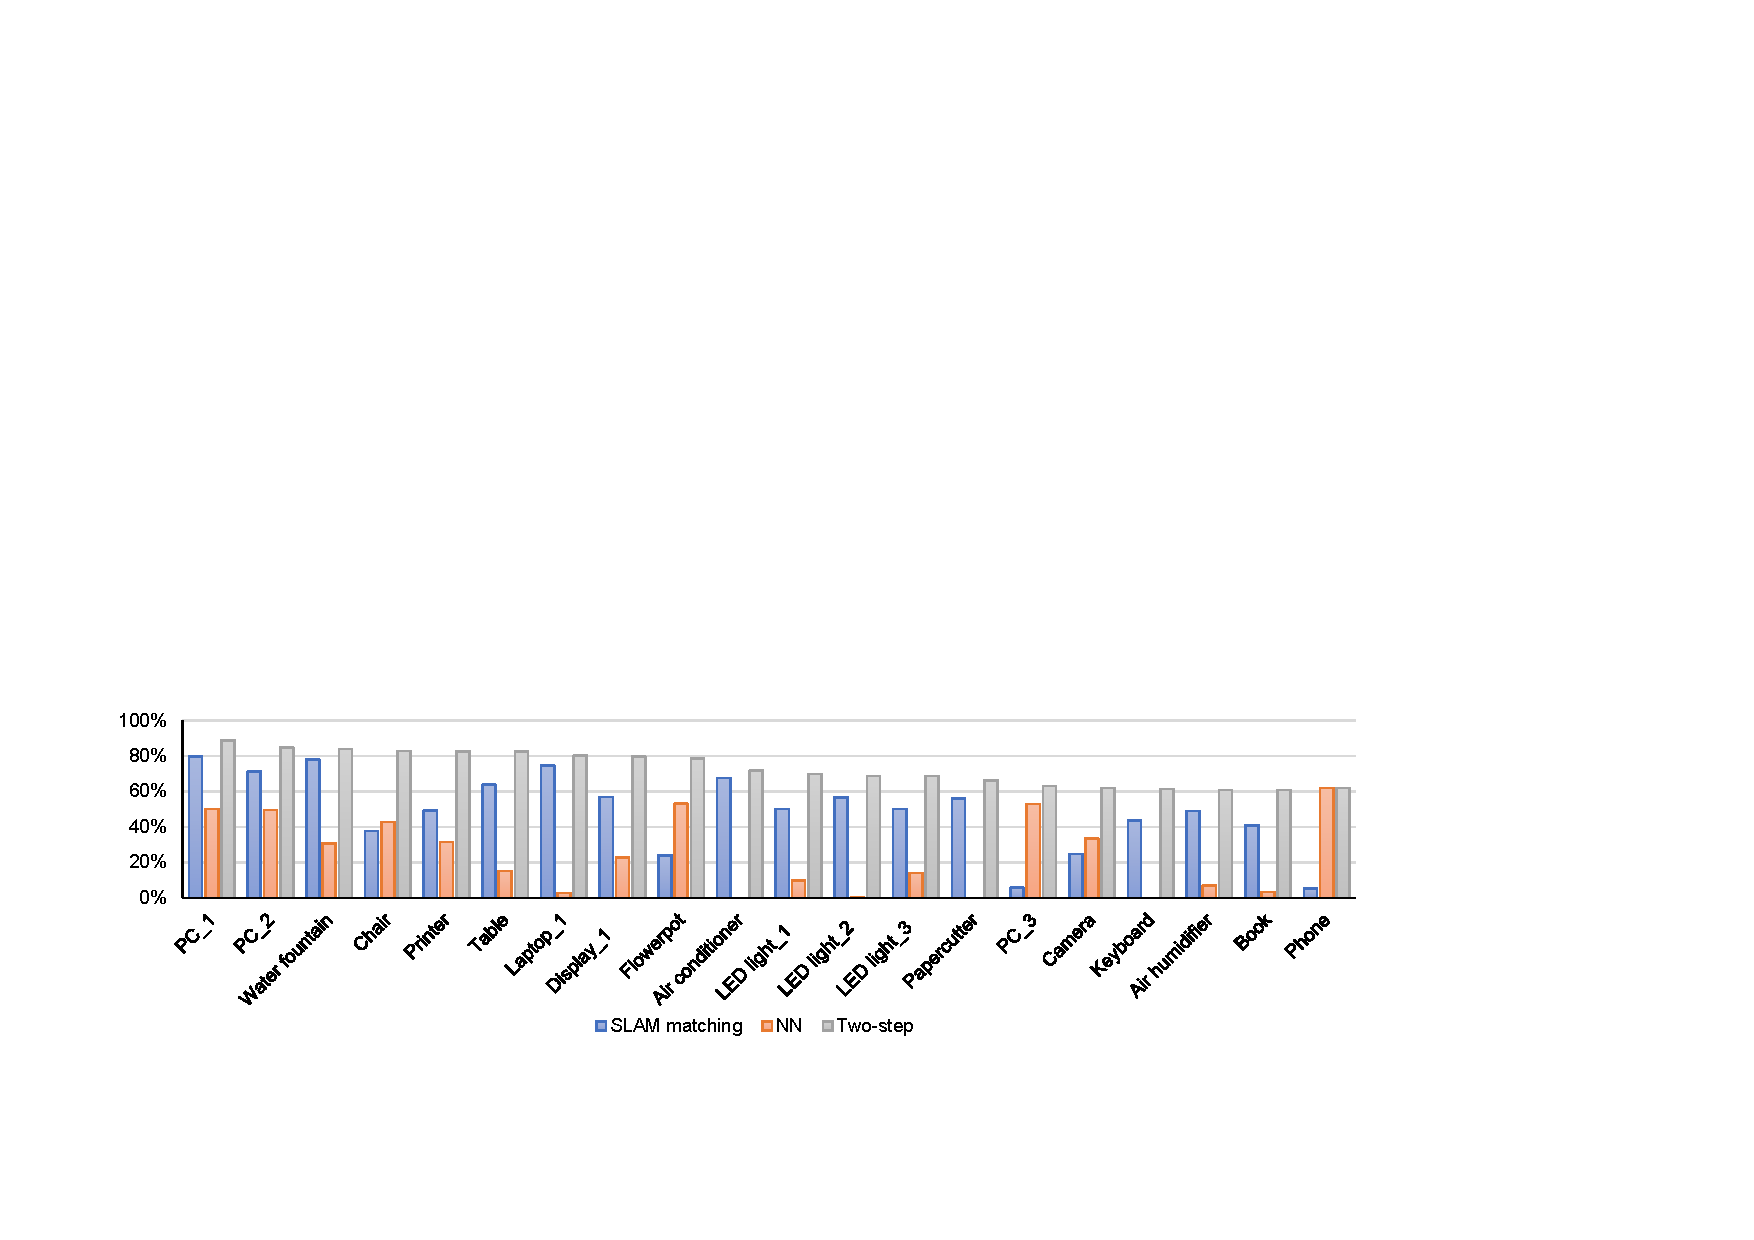
\includegraphics[width=0.95\linewidth]{ident-res}
	\caption{使用子图后目标检测延迟的改善}
	\label{fig:identification}
\end{figure*}

\textbf{VSLink的识别准确率}: 
我们计算了VSLink的识别精度,并将结果绘制在\autoref{fig:identification}中。我们可以看到,平均两阶段识别准确率达到72.7\%。对于基于SLAM匹配的方法,平均精度为49.2\%,而对于只基于神经网络的方法,平均精度为44.7\%。这两种方法互为补充,实现了多目标识别。在这里,我们没有针对这种情况对神经网络进行再训练,因为我们希望它是通用的,并且我们认为在使用专门的神经网络时它应该会表现出更好的性能。

我们认为漏检可分为两种情况。
一是我们在SLAM匹配和神经网络检测方面都失败了,所以我们需要考虑1)训练更好的神经网络,2)重建地图,让这个对象有更多的附着的地图点。
非常小的物体对于VSLink来说是极大的挑战,因为它们不容易被神经网络检测到。
我们希望通过神经网络的改进提高对小目标检测的能力,学术界对此正在进行研究,并且取得了一定进展。

\textbf{移动物体的识别}: 
对于第四次/第五次视频,我们手动移动了六个对象,包括三个稳定的对象和三个可移动的对象。
对于稳定的对象,我们将它们移动了一小段距离(小于50厘米)。对于可移动的物体,我们将它们移动了很长的距离(超过2米)。
我们测试了VSLink是否可以重新识别移动的对象。
结果表明,该方法对稳定物体的识别准确率为83\%,对可移动物体的识别准确率为66\%。
由于我们依靠神经网络进行运动目标检测,这就要求我们采用更先进、更精确的网络。


\textbf{鲁棒性}: 
我们通过五天的使用评估了VSLink的鲁棒性。在第四天和第五天,我们在环境中手动移动了一些对象。
结果显示,在最后一天,识别准确率下降了10\%。我们分析了数据,发现基于SLAM匹配的识别在不同的光照条件或环境变化时出现了更多的未匹配点。这意味着我们需要随着时间的推移主动更新地图,否则地图会随时间流逝而逐渐失效。
而时间因素通常不会影响基于神经网络的检测的鲁棒性。

在我们的实现中,我们还没有实现地图实时更新的方法,但我们认为这是可行的。地图实时更新面临的挑战是主动更新地图点并对其进行标记,这需要执行实例分割神经网络,并且需要花费大量时间。
我们可以应该让我们的主线程,即两阶段对象识别过程,占用主要的计算资源。
地图更新线程以延后的方式执行。

\subsection{案例验证}
演示VSLink在人机交互方面的能力。在这里,我们在\autoref{fig:cases}中展示了由VSLink开发的三个应用程序。第一个是智能会议室,我们将VSLink连接到会议室的设备,并设计相应的UI。用户可以通过VSLink控制门、投影仪、扬声器和空调。
二是植物养护。对于养植物的用户,我们设计了交互功能来记录浇水时间和浇水量,并记录重要日期,如开花日。
三是设备管理。对于实验室中的公共设备,我们记录并显示其元数据,如正式用户、当前用户、数据表等。此功能有助于管理大型设备。
我们要求10名志愿者评估VSLink的定制交互设计。
志愿者都是校园里的学生。
我们要求他们为随机选择的对象设计UI。
在实验中,他们平均需要两分钟即可完成设计。

\begin{figure}[t]
	\centering
	\begin{subfigure}{.65\linewidth}
		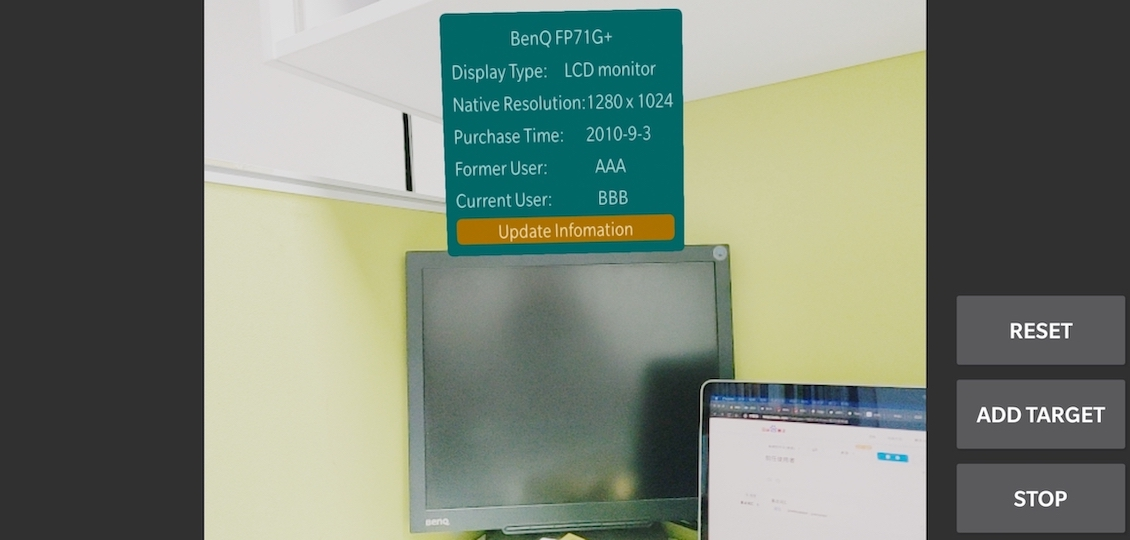
\includegraphics[width=1\linewidth]{case1}
		\caption{}
	\end{subfigure}
	%\hskip2em\
	%\centering
	\begin{subfigure}{.65\linewidth}
		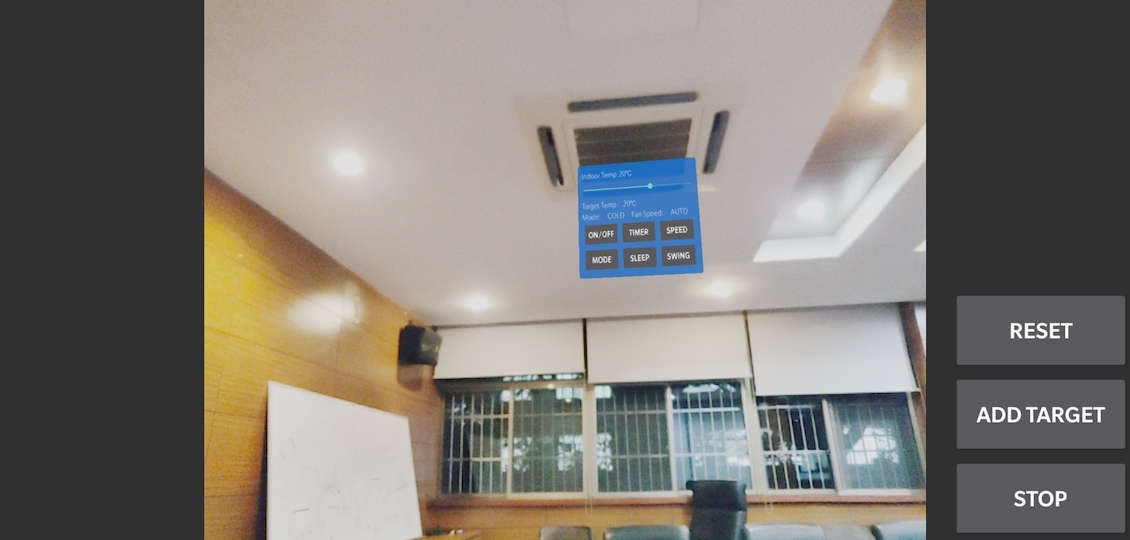
\includegraphics[width=1\linewidth]{case2}
		\caption{}
	\end{subfigure}
	\begin{subfigure}{.65\linewidth}
		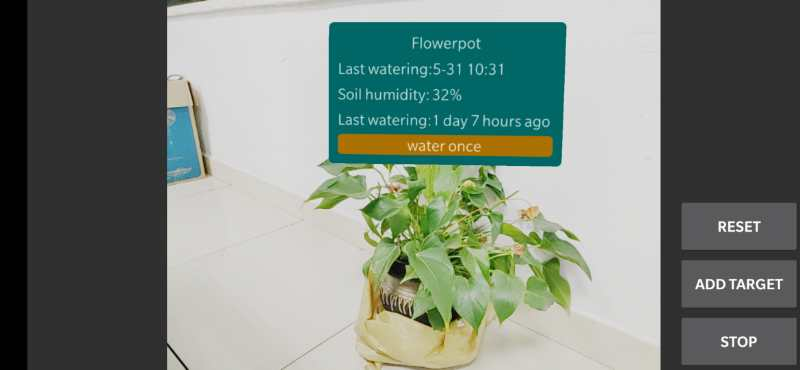
\includegraphics[width=1\linewidth]{case3}
		\caption{}
	\end{subfigure}
	\caption{三个VSLink实现的应用}\label{fig:cases}
\end{figure}


\section{相关工作}\label{sec:related}
现有的人机交互方法主要分为基于视觉的方法和其他方法。

\textbf{基于视觉的方法}: 
利用深度学习的进步,计算机视觉在支持人机交互方面取得了巨大的进步。
视觉标记\cite{wang2010design,olson2011apriltag}在日常生活中非常实用,它将物理对象与电子信息结合在一起,并帮助我们区分具有非常相似外观的对象。但是,它有一些限制,因为1)它会影响对象的外观,2)它需要用户调整相机焦距以识别标记。
另一个通用框架是目标检测\cite{ren2015faster,redmon2018yolov3,qin2019thundernet}和图像检索\cite{philbin2008lost,zheng2017sift}的组合。然而,单次推理的延迟过高是阻碍该方法实际应用的关键性弱点。
商用AR系统ARcore\cite{arcore}和ARkit\cite{arkit}已经展示出了其辅助人机交互的能力。
它们使用SLAM技术来理解环境,然后他们可以帮助用户以自然的方式放置虚拟元素。但问题在于它们无法识别对象,因为它们没有关于真实对象的信息。因此,他们只能记住虚拟元素的位置,而不能真正将其与真实对象绑定,这使得环境一旦发生改变,它们就会丢失它们的绑定关系。
Snap-to-it\cite{de2016snap}和SnapLink\cite{chen2018snaplink}要求用户拍摄目标设备的照片以进行识别,一次录入一个设备。
这种实现可能会限制用户的使用场景并损害用户体验。例如,当用户到达一个新的地方时,他可能需要花费大量的精力来首先确定哪些对象可以与之交互。
高级语义SLAM技术~\cite{strecke2019fusion,runz2018maskfusion,salas2013slam++}可以用于人机交互,但它们没有考虑到地图重用,而地图重用是基于SLAM的对象识别的关键。
\cite{liu2019edge}研究了边缘辅助的实时移动AR,实现了较高的帧率。但是对于人机交互,\cite{liu2019edge}仍然缺乏识别设备的能力。
\cite{ben2020edge,xu2020edge,liu2021edgesharing}提出了边缘辅助SLAM,实现了实时的移动SLAM。这可以用于实现基于AR的人机交互,但还需要进一步的集成工作。

\textbf{其他基于感知的技术}: 
Physical web\cite{jenson2014physical}允许蓝牙设备和带有beacon(信标)的对象广播智能手机可以接收的URL。附近的用户可以通过访问URL访问其界面。
该方法实现了快速准确的目标发现,但交互形式仍然是传统的。
与基于AR的解决方案相比,它缺乏直观和丰富的信息显示能力。
Summon\cite{zachariah2020browsing}设计了一种用于与可连接对象交互的浏览技术,但它具有与Physical web类似的限制。
为了完成这项任务,还研究了一些射频和声学技术\cite{alanwar2017selecon,pu2013whole,mao2016cat}。
Selecon\cite{alanwar2017selecon}使用基于UWB的定位技术来实现设备选择和控制系统。
然而,需要使用专用设备的要求限制了其实际应用。
基于语音的解决方案具有自然和无需手持交互的优势,特别是当用户没有手持智能手机时。另一方面,与基于AR的解决方案相比,它的交互速度和丰富性较弱。

总而言之,现有的人机交互尝试仍然不能提供令人眼前一亮的人机交互。
与之相比,VSLink通过提出的关键技术提高了交互能力、速度和用户体验。

\section{总结}\label{sec:sum}
在本文中,我们提出了VSLink,这是一种基于视觉技术的方法,用于实现与环境对象的快速和普适交互。
在VSLink中,我们利用视觉SLAM识别对象,并加速对象检测神经网络,使总延迟小于33ms。VSLink还为用户提供了一个平台,以实现面向用户的交互,其中自定义UI是以无代码的方式开发的。
我们在包含多个要交互的对象的环境中评估了VSLink。结果表明,该算法在30fps的视频输入下具有良好的性能,目标识别率为{\acc}。

% \chapter{参考命令}
% \section{节标题}

% 我们可以用includegraphics来插入现有的jpg等格式的图片,
% 如\autoref{fig:zju-logo}所示。

% \begin{figure}[htbp]
%     \centering
%     \includegraphics[width=.3\linewidth]{logo/zju}
%     \caption{\label{fig:zju-logo}浙江大学LOGO}
% \end{figure}


% \subsection{小节标题}


% \par 如\autoref{tab:sample}所示,这是一张自动调节列宽的表格。

% \begin{table}[htbp]
%     \caption{\label{tab:sample}自动调节列宽的表格}
%     \begin{tabularx}{\linewidth}{c|X<{\centering}}
%         \hline
%         第一列 & 第二列 \\ \hline
%         xxx & xxx \\ \hline
%         xxx & xxx \\ \hline
%         xxx & xxx \\ \hline
%     \end{tabularx}
% \end{table}


% \par 如\autoref{equ:sample},这是一个公式

% \begin{equation}
%     \label{equ:sample}
%     A=\overbrace{(a+b+c)+\underbrace{i(d+e+f)}_{\text{虚数}}}^{\text{复数}}
% \end{equation}

% \chapter{另一章}

% \begin{figure}[htbp]
%     \centering
%     \includegraphics[width=.3\linewidth]{example-image-a}
%     \caption{\label{fig:fig-placeholder}图片占位符}
% \end{figure}